\documentclass[pdf]{beamer}
\mode<presentation>{} 

\usepackage{hyperref}
\usepackage{pgf}
\usepackage{tikz}
\usetikzlibrary{trees}
\usetikzlibrary{arrows,automata}
\usetikzlibrary{automata,positioning}
\usetikzlibrary{shapes}
\usepackage{tikz-qtree,tikz-qtree-compat}
\usepackage{mathtools,enumerate,amssymb}
\usepackage[utf8]{inputenc}
\usepackage[T1]{fontenc}
\usepackage{graphicx}

\title{Introducere in teoria limbajelor formale}
\subtitle{Limbaje formale şi translatoare (Compilatoare)}
\AtBeginSection[]{}

\setbeamertemplate{sidebar right}{}
\setbeamertemplate{footline}{%
\hfill\usebeamertemplate***{navigation symbols}
\hspace{1cm}\insertframenumber{}/\inserttotalframenumber}

\begin{document}

\begin{frame}
	\titlepage
	
\begin{flushright}
Mihai-Lica Pura\\
\end{flushright}

\end{frame}



\begin{frame}{Cuprins}
\begin{itemize}
\item
Introducere: Definiție, importanță, istoric
\item
Gramatici formale
\item
Arbori de analiză gramaticală
\item
Limbaje regulare
\begin{itemize}
\item
automate finite
\item
expresii regulare
\end{itemize}
\item
Limbaje independente de context
\begin{itemize}
\item
automate finite cu stivă
\end{itemize}
\end{itemize}
\end{frame}



\begin{frame}{Definiția limbajului}
\begin{itemize}
\item
Știința care se ocupă cu studiul limbajelor (naturale) se numește \textit{lingvistică}.
\item
Limbajul este un sistem de comunicare bazat pe cuvinte și pe combinarea cuvintelor pentru a forma propoziții și fraze.
\begin{itemize}
\item
fonologia - regulile după care simbolurile sunt utilizate pentru a forma cuvinte sau morfeme (microsintaxă)
\item
sintaxa - regulile după care cuvintele sau morfemele se combină pentru a forma propoziții și fraze
\item
semiotică - procesul prin care semnele sunt legate de anumite înțelesuri (semantică)
\end{itemize}
\end{itemize}
\end{frame}



\begin{frame}{Definiția limbajului}
\begin{itemize}
\item
Comunicarea înseamnă schimbul de informații, cunoștințe, credințe, opinii, dorințe, ordine, amenințări, mulțumiri, promisiuni, declarații, sentimente, etc.
\item
Clasificare
\begin{itemize}
\item
Comunicare lingvistică - bazată pe un limbaj
\item
Comunicare non-lingvistică - zâmbetul, râsul, strigatul, ridicatul din umeri, etc.
\end{itemize}
\end{itemize}
\end{frame}



\begin{frame}{Importanța limbajului}
\begin{itemize}
\item
Limbajul arată felul în care noi percepem realitatea
\item
De exemplu: 
\begin{itemize}
\item
în limba română spunem: 

\textit{Avionul zboară pe cer.}

\item
în limbile franceză şi engleză spunem:

\textit{L’avion vole dans le ciel.}

\textit{The plane flies in the sky.}
\end{itemize}
\item
Iar acest lucru se regăseşte şi în felul în care au fost proiectate limbajele formale, adică felul în care noi prezentăm realitatea calculatoarelor
\end{itemize}
\end{frame}



\begin{frame}{Importanța limbajului}
\begin{figure}[ht!]
\centering

\includegraphics[scale=0.18]{img/arrivalposter.jpg}
\end{figure}
\end{frame}



\begin{frame}{Importanța limbajului}
\begin{itemize}
\item
Versiunea "Weltanschauung" extremă a ipotezei Sapir-Whorf
\item
Determinismul lingvistic
\begin{itemize}
\item
structura unui limbaj influențează sau determină percepția asupra lumii
\item
percepția asupra lumii
\begin{itemize}
\item
descrie consistent și integral existența
\item
oferă cadrul de lucru teoretic pentru a genera, susține și aplica cunoașterea
\end{itemize}
\end{itemize}
\end{itemize}
\end{frame}



\begin{frame}{Paradigme de programare}
\textbf{Programarea structurată}
\begin{itemize}
\item
paradigmă de programare axată pe îmbunătăţirea calităţii, clarităţii şi timpului de dezvoltare a codului unui program, prin utilizarea in extenso a \textbf{funcţiilor (subrutinelor), blocurilor de instrucţiuni, şi a instrucţiunilor repetitive (for, while, ş.a.)}
\item
versus
\item
utilizarea salturilor de tipul \textbf{goto}, care produc un cod dezordonat (spaghetti), care este foarte greau de întreţinut şi de depanat
\item
Exemple: C, C++, C\#, Java, ş.a.
\end{itemize}
\end{frame}



\begin{frame}{Paradigme de programare}
\textbf{Programarea imperativă}
\begin{itemize}
\item
paradigmă de programare care descrie computaţiile în termeni de \textbf{enunţuri} care modifică \textbf{starea} programului
\item
seamănă \textbf{modului imperativ} din limbajul natural, prin care enunţăm \textbf{comenzi} care cer efectuarea unor anumite acţiuni
\item
programele imperative definesc succesiuni de comenzi, care să fie executate de către computer
\item
Exemple: C, C++, C\#, Java, ş.a.
\end{itemize}
\end{frame}



\begin{frame}[fragile]
\frametitle{Paradigme de programare}
\textbf{Bubble sort în C}
\begin{verbatim}
void bubble_sort(long list[], long n) {
  long c, d, t;
  for (c = 0 ; c < ( n - 1 ); c++) {
    for (d = 0 ; d < n - c - 1; d++) {
      if (list[d] > list[d+1])
      {
        t         = list[d];
        list[d]   = list[d+1];
        list[d+1] = t;
      }
    }
  }
}
\end{verbatim}
\end{frame}



\begin{frame}{Paradigme de programare}
\textbf{Programarea declarativă}
\begin{itemize}
\item
paradigmă de programare care exprimă logica unei computaţii, fără a descrie fluxul ei de control
\item
vine în contraponderea paradigmei imperative, care are nevoie de un algoritm explicit precizat
\item
scopul este minimizarea şi chiar eliminarea efectelor secundare, descriind \textbf{ceea ce} trebuie să facă un program, iar nu \textbf{cum} trebuie să procedeze pentru a face acel lucru
\item
Exemple: limbaje de programare funcţionale (vezi slide-ul următor), limbaje de programare logice (Prolog, ş.a.)
\end{itemize}
\end{frame}



\begin{frame}{Paradigme de programare}
\textbf{Programarea funcţională}
\begin{itemize}
\item
paradigmă de programare care defineşte computaţia ca o evaluare a unor funcţii matematice şi care evită folosirea stării şi a variabilelor
\item
este bazată pe aplicarea funcţiilor, spre deosebire de paradigma imperativă care este bazată pe schimbările stării programului
\item
Exemple: Haskell, Scala, F\#, ş.a.
\end{itemize}
\end{frame}



\begin{frame}[fragile]
\frametitle{Paradigme de programare}
\textbf{Bubble sort în Scala}
\begin{verbatim}
def bubblesort[A <% Ordered[A]](list: List[A]):List[A] = {
  def sort(as: List[A], bs: List[A]): List[A] =
    if (as.isEmpty) bs
    else bubble(as, Nil, bs)

  def bubble(as: List[A], zs: List[A], bs: List[A]):List[A] 
    = as match {
      case h1 :: h2 :: t =>
        if (h1 > h2) bubble(h1 :: t, h2 :: zs, bs)
        else bubble(h2 :: t, h1 :: zs, bs)
      case h1 :: Nil => sort(zs, h1 :: bs)
  }
  
  sort(list, Nil)
}
\end{verbatim}
\end{frame}



\begin{frame}{Paradigme de programare}
\textbf{Programarea orientată pe obiecte}
\begin{itemize}
\item
paradigmă de programare care foloseşte pentru computaţii obiectele (de obicei instanţe ale unei clase)
\item
un obiect constă din gruparea unor atribute (câmpuri de date) şi a unor metode şi a interacţiunii dintre ele
\item
permite utilizarea unor tehnici de programare ca: abstractizarea, încapsularea, polimorfismul, moştenirea, ş.a.
\item
Exemple: C++, C\#, Java, ş.a.
\end{itemize}
\end{frame}



\begin{frame}{Paradigme de programare}
\textbf{Programarea event-driven}
\begin{itemize}
\item
paradigmă de programare în care fluxul programului este determinat de evenimente (înregistrarea unor valori de către senzori; acţiunile utilizatorului - clic cu mouse-ul, apăsarea unei taste, etc.; recepţionarea unor mesaje de la alte fire de execuţie sau de la alte programe)
\item
Exemple: C Win32 API
\end{itemize}
\end{frame}



\begin{frame}{Paradigme de programare}
\textbf{Metafizica limbajelor de programare}
\begin{itemize}
\item
Platon, în opera \textit{Republica} descrie noțiunea de \textbf{lume a ideilor}: toate lucrurile din univers au un corespondent abstract în lumea ideilor
\item
de exemplu, o masă din lumea reală este doar o reflexie imperfectă a ideii de Masă din lumea idelor
\item
elementele abstracte din lumea ideilor se constituie într-o ierarhie de tipuri, care are ca și rădăcină un tip suprem
\item
scopul filosofului este a descoperi care este acest tip suprem din care sunt derivate toate cele care există
\end{itemize}
\end{frame}



\begin{frame}{Paradigme de programare}
\textbf{Metafizica limbajelor de programare}
\begin{itemize}
\item
Platon - alegoria peșterii - tipul suprem este bunătatea
\item
neoplatonicii - tipul suprem este Dumnezeu
\item
programarea orientată pe obiecte - tipul suprem este clasa din care sunt derivate toate celelalte clase
\item
C\# și Java oferă o percepție platonică asupra lumii, având clasa \textit{Object} din care sunt derivate toate celelalte clase
\end{itemize}
\end{frame}



\begin{frame}{Paradigme de programare}
\textbf{Metafizica limbajelor de programare}
\begin{itemize}
\item
Aristotel în \textit{Fizica} consideră că fiecare obiect din univers este construit folosind elemente primitive discrete numite atomi
\item
de exemplu, pentru a construi o masă: 
\begin{itemize}
\item
este nevoie ca atomii să se aranjeze în ordinea corectă pentru a forma lemnul 
\item
iar apoi, elementele de lemn sunt aranjate pentru a crea masa
\end{itemize}
\item
limbajele de programare aristoteliene sunt cele care se bazează pe primitive discrete (char, int, float, double) pe baza cărora construiesc apoi elemente din ce în ce mai complexe
\item
de exemplu: pentru a reprezenta un șir de caractere se folosește un vector de tip char, iar nu o clasă de tip string
\end{itemize}
\end{frame}



\begin{frame}{Istoria limbajului - creaţia}
\begin{itemize}
\item
Istoria culturală a tuturor popoarelor a consemnat preocuparea pentru “limba perfectă” (până în sec. XVII-lea)
\item
Prima variantă: \textbf{Dumnezeu i-a dat lui Adam o formă a limbii ebraice (perfecte)}, prin care El i-ar fi vorbit lui Adam:

\textit{“A dat apoi Domnul Dumnezeu lui Adam poruncă şi a zis: "Din toţi pomii din rai poţi să mănânci, Iar din pomul cunoştinţei binelui şi răului să nu mănânci, căci, în ziua în care vei mânca din el, vei muri negreşit!”} (Geneza, 2:16-17)
\end{itemize}
\end{frame}



\begin{frame}{Istoria limbajului - creaţia}
\begin{itemize}
\item
A doua variantă: \textbf{Adam ar fi inventat-o dând un nume animalelor}:

\textit{“Şi Domnul Dumnezeu, Care făcuse din pământ toate fiarele câmpului şi toate păsările cerului, le-a adus la Adam, ca să vadă cum le va numi; aşa ca toate fiinţele vii să se numească precum le va numi Adam. Şi a pus Adam nume tuturor animalelor şi tuturor păsărilor cerului şi tuturor fiarelor sălbatice.”} (Geneza, 2:19-20)
\item
Şi în care ar fi avut primul dialog cu Eva.
\end{itemize}
\end{frame}



\begin{frame}{Istoria limbajului - creaţia}
\begin{itemize}
\item
A treia variantă: \textbf{Dumnezeu i-a dat lui Adam o gramatică generală}, o formă transcedentală cu care să construiască toate limbile posibile ("De Vulgari Elequentia", Dante).
\begin{itemize}
\item
\textbf{Dumnezeu Chomskyan} i-a dat lui Adam nişte structuri sintactice profunde, ce se regăsesc în orice limbă creată ulterior de către oameni.
\item
Dumnezeu i-a dat lui Adam (Adam a identificat în construirea primei limbi) nişte \textbf{universalii semantice - un sistem de noţiuni atomice} - prin combinarea cărora se poate da seamă de întreg mobilierul universului.
\end{itemize}
\end{itemize}
\end{frame}



\begin{frame}{Istoria limbajului - apariţia limbilor popoarelor}
\begin{itemize}
\item
\textit{"În vremea aceea era în tot pământul o singură limbă şi un singur grai la toţi."}(Geneza, 11: 11)
\item
\textbf{Versus}
\item
\textit{"Din acestia [fii lui Noe] s-au format mulţime de popoare, care s-au aşezat în diferite ţări, fiecare după limba sa, după neamul său şi după naţia sa."}(Geneza, 10: 5)
\item
\textit{"Aceştia sunt fiii lui Ham, după familii, limbă, ţări şi după naţii."}(Geneza, 10: 20)
\item
\textit{"Acestia sunt fiii lui Sem după familii, după limbă, după ţări şi după naţii."}(Geneza, 10: 31)
\end{itemize}
\end{frame}



\begin{frame}{Istoria limbajului - Gândire şi limbaj}
\begin{itemize}
\item
Iniţial se credea că există o gramatică universală a ideilor care reflectă însăşi organizarea universului.
\item
Implică faptul că există o structură de noţiuni universale prezente în limba şi în gândirea oricarui popor.
\item
Există deci un sistem al ideilor, acelaşi pentru toţi oamenii, iar de la popor la popor aceleiaşi idei i se dau nume diferite.
\item
Ex: ideogramele chinezeşti
\begin{itemize}
\item
aceleaşi pentru chinezi, japonezi şi coreeni
\item
pronunţate cu sunete diferite pentru fiecare popor în parte
\item
trimit la aceleaşi concepte (pentru aceste popoare diferite)
\end{itemize}
\end{itemize}
\end{frame}



\begin{frame}{Istoria limbajului - Inventarea unui limbaj}
\begin{itemize}
\item
Inventarea unor limbi (ulterior numite filosofice şi a priori) – ele nu sunt descoperite, ci construite pe baza unei viziuni filosofice asupra lumii.\\
\item
Scopurile căutării anterioare:
\begin{itemize}
\item
Convertirea necredincioşilor la creştinism,\\
\item
Regăsirea comuniunii mistice cu Dumnezeu şi cu lucrurile pe care le însemna limba perfectă a lui Adam.
\end{itemize}
\item
Scopurile invenţiilor:
\begin{itemize}
\item
Favorizarea schimburilor comerciale,
\item
Pătrunderea colonială,
\item
Răspândirea ştiinţei.
\end{itemize}
\end{itemize}
\end{frame}



\begin{frame}{Istoria limbajului - Inventarea unui limbaj}
\begin{itemize}
\item
“Common writing”, Lodwick (1647)
\item
“Ars Signorum”, Dalgarnus (1661)
\item
“Essay Towards a Real Character”, John Wilkins (1668)
\newline
\item
“Les estats et les empires de la lune”, Cyrano de Bergerac
\item
“Les estats et les empires du soleil”, Cyrano de Bergerac
\item
“The Man in the Moon”, Francis Godwin
\item
“La terre australe connue”, Gabriel de Foigny
\item
“L’Histoire des Sevarambes”, Deinis Veiras
\end{itemize}
\end{frame}



\begin{frame}{Limbaje formale}
\begin{itemize}
\item
FORMÁL, -Ă, formali, -e, adj. 
\begin{enumerate}
\item
Privitor la formă, care ține de formă, de aparență. (Adverbial) În aparență. 
\item
Formulat precis; categoric, expres. 
\item
Pătruns de formalism; făcut de formă (7). 
\item
(Despre unele acte juridice) Care necesită anumite forme pentru a fi socotit legal și valabil.
\end{enumerate}
(dexonline)
\item
Limbajele naturale nu se bazează pe reguli stricte
\item
Rezultatul: \textit{ambiguitatea semnatică} - același cuvânt sau aceeași propoziție/construcție/frază poate să aibă mai multe înțelesuri, adică poate să fie interpretată în mai multe moduri
\end{itemize}
\end{frame}



\begin{frame}{Limbaje formale}
\begin{figure}[ht!]
\centering
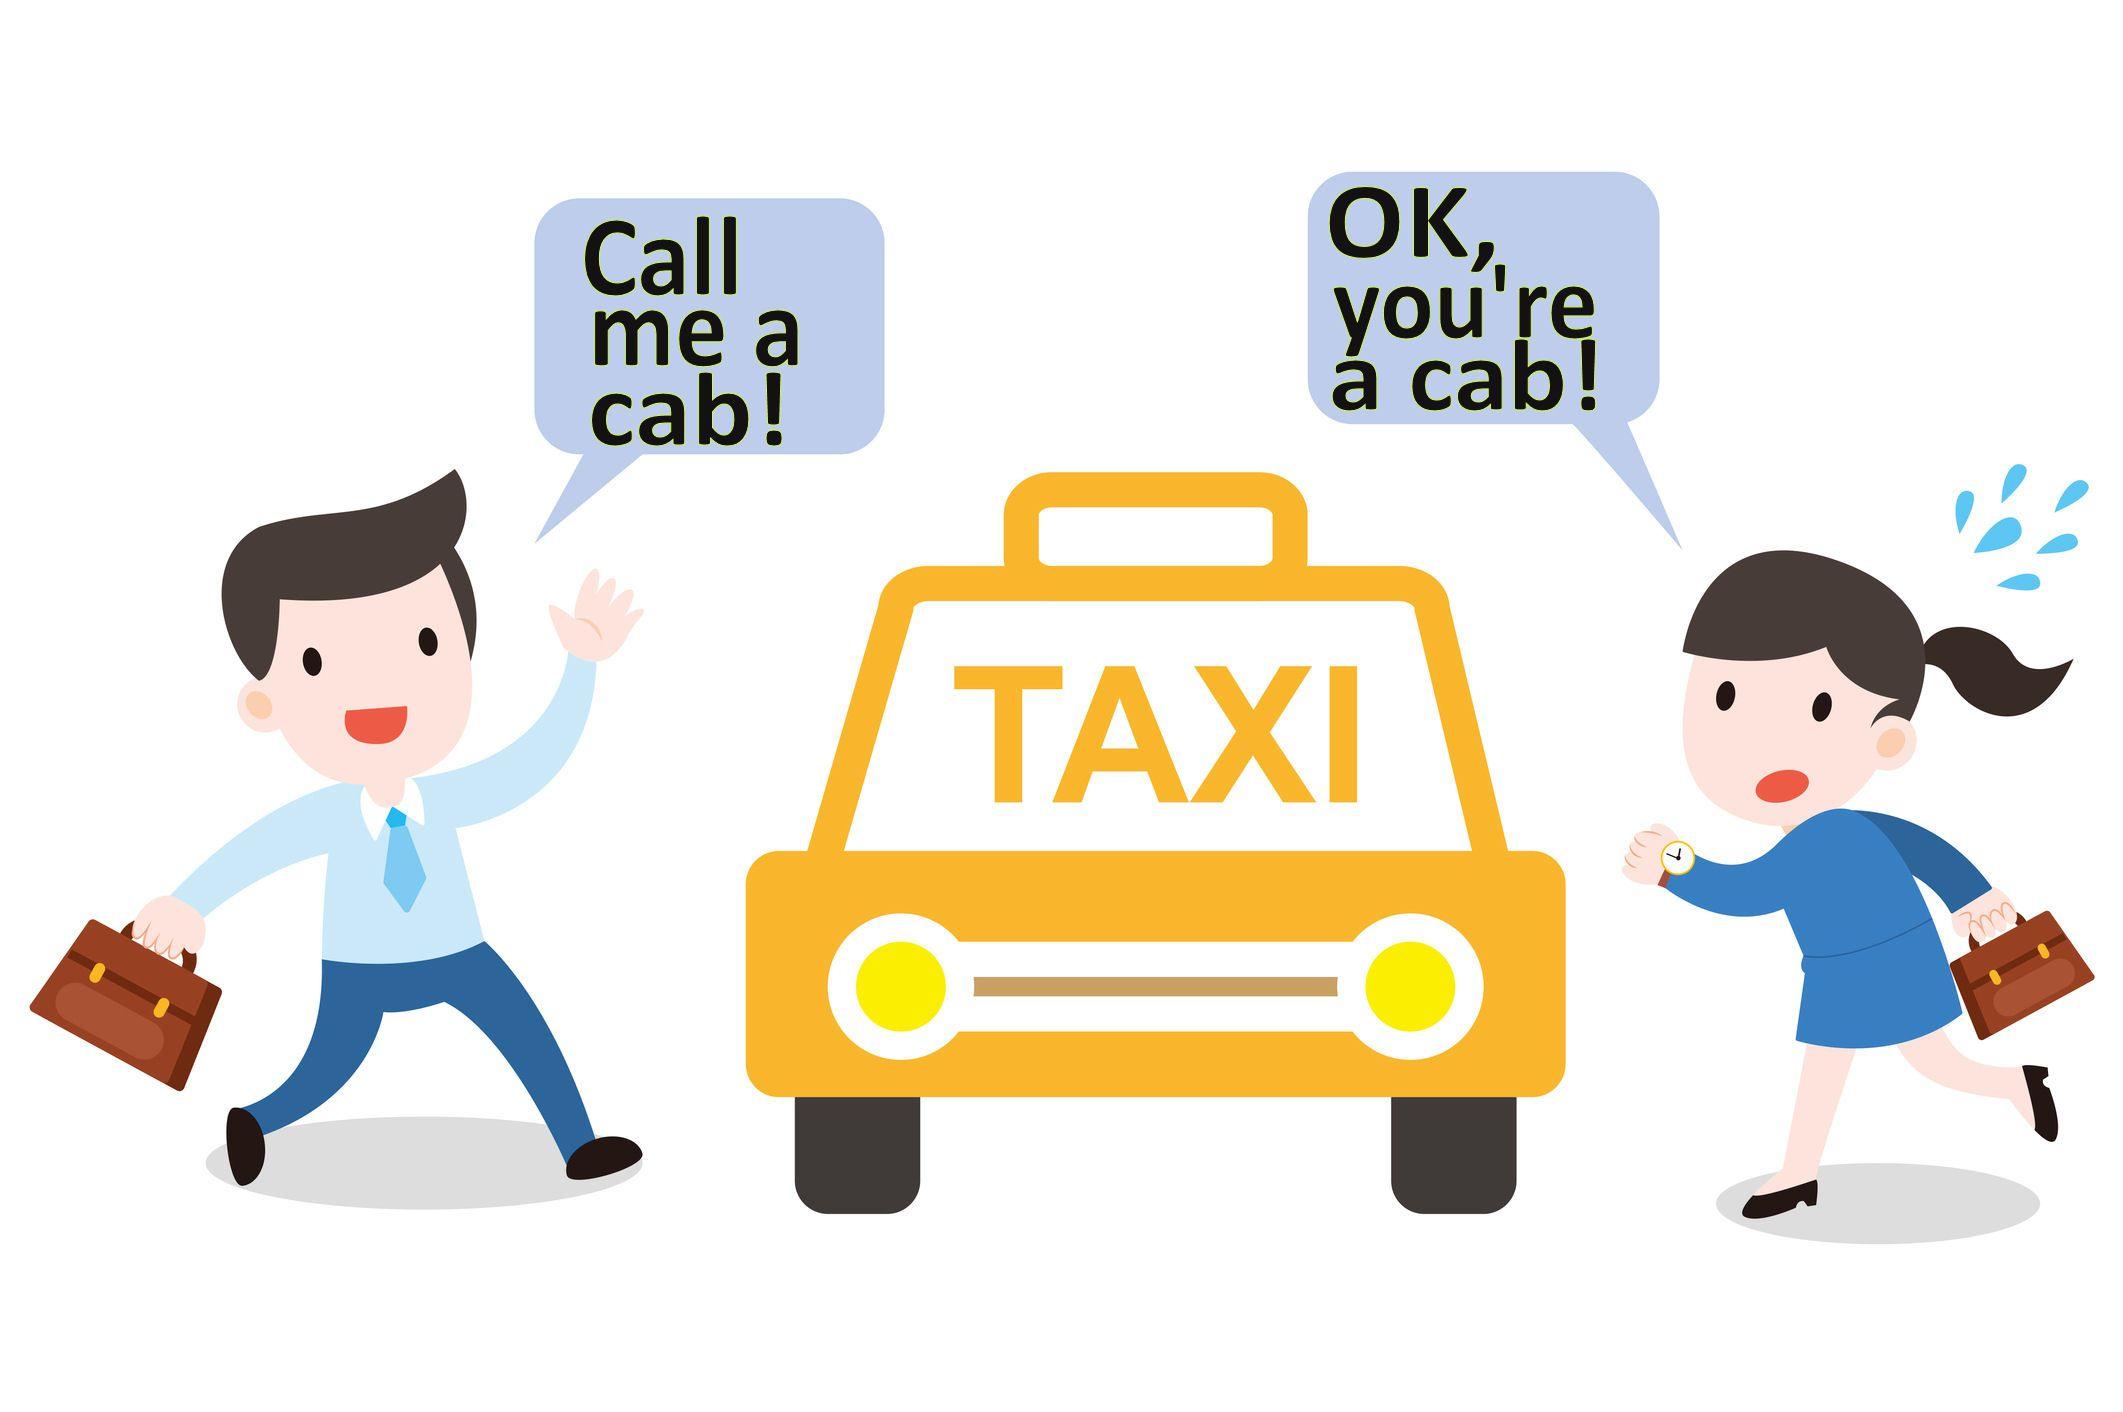
\includegraphics[scale=0.1]{img/callmeacab.jpg}
\end{figure}
\end{frame}



\begin{frame}{Limbaje formale}
\begin{itemize}
\item
pentru oameni, acest lucru nu constituie neapărat o problemă
\item
oamenii deduc sensul imediat folosindu-se de context
\begin{figure}[ht!]
\centering
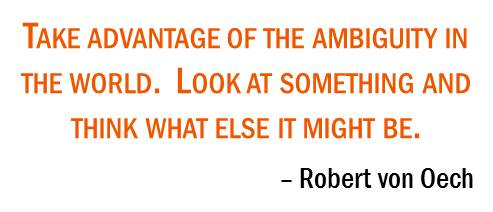
\includegraphics[scale=1]{img/Ambiguity-Quote-Image.jpg}
\end{figure}
\item
pentru calculatoare, ambiguitatea este o problema - soluția limbajele formale
\end{itemize}
\end{frame}



\begin{frame}{Limbaje formale}
\begin{itemize}
\item
Limbajul este o modalitate sistematică de comunicare care utilizează sunete sau \textit{simboluri convenţionale}. 
\item
În cazul limbajelor de programare, simbolurile convenţionale sunt \textit{şiruri de caractere}.
\item
Pentru a defini un şir de caractere trebuie să pornim de la un alfabet.
\end{itemize}
\end{frame}



\begin{frame}{Limbaje formale}
\begin{itemize}
\item
Un \textbf{alfabet} este o mulţime finită de simboluri.
\item
Exemple:
\begin{itemize}
\item
$\Sigma_{1} = \{$a, ă, â, b, c, d, $\dots$, z$\}$ este mulţimea literelor din alfabetul limbii române.
\item
$\Sigma_{2} = \{$0, 1, $\dots$, 9$\}$ este mulţimea cifrelor în baza 10.
\item
$\Sigma_{3} = \{$a, b, $\dots$, z, \# $\}$ este mulţimea literelor din alfabetul latin, plus simbolul special $\#$.
\end{itemize}
\end{itemize}
\end{frame}



\begin{frame}{Limbaje formale}
\begin{itemize}
\item
O succesiune finită de simboluri din alfabetul $\Sigma$ se numeşte \textbf{şir de simboluri} peste alfabetul dat.
\item
Exemple:
\begin{itemize}
\item
\textit{abfbz} este şir de caractere peste $\Sigma_{1} = \{$a, b, c, d, $\dots$, z$\}$,
\item
\textit{9021} este şir de caractere peste $\Sigma_{2} = \{$0, 1, $\dots$, 9$\}$,
\item
\textit{ab\#bc} este şir de caractere peste $\Sigma_{3} = \{$a, b, $\dots$, z, \#$\}$.
\end{itemize}
\item
Un \textbf{limbaj} este o mulţime de şiruri (finită sau infinită) de simboluri peste acelaşi alfabet.
\end{itemize}
\end{frame}



\begin{frame}{Limbaje formale}
\begin{itemize}
\item
Dacă limbajul este finit atunci el poate să fie definit prin \textbf{enumerare}. 
\item
Dacă limbajul este infinit atunci există două mecanisme de definire: 
\begin{itemize}
\item
prin \textbf{generare} 
\begin{itemize}
\item
gramaticile formale
\item
ştie să genereze toate propoziţiile din limbaj (şi numai pe acestea), astfel încât alegând o propoziţie din limbaj, va ajunge sa genereze propoziţia respectivă într-un interval finit de timp
\end{itemize}
\item
prin \textbf{recunoaştere}
\begin{itemize}
\item
automatele finite și expresiile regulare
\item
ştiu să recunoască (să accepte ca fiind corecte) propoziţiile limbajului dat (şi numai pe acestea)
\end{itemize}
\end{itemize}
\end{itemize}
\end{frame}



\begin{frame}{Gramatici formale}
\textbf{Cuprins}
\begin{itemize}
\item
Intuiție
\item
Definiție
\item
Relația de derivare
\begin{itemize}
\item
derivarea directă
\item
derivarea în k pași
\item
închiderea tranzitivă a relației de derivare
\item
închiderea tranzitivă și reflexivă a relației de derivare
\end{itemize}
\item
formă propozițională
\item
propoziție
\item
limbaj
\item
Ierarhia Chomsky. Tipuri de gramatici formale
\end{itemize}
\end{frame}



\begin{frame}{Gramatici formale}
\textbf{Intuiție}
\begin{itemize}
\item
fie o mulţime de cuvinte:

\textit{ \{ casa, străluceşte, rapid, copila, stă, frumos, câinele, aleargă, alb \} }
\item
să formăm propoziţii de câte trei cuvinte alese la întâmplare, care să aibă înţeles în limba română
\item
evident, avem toate şansele de a forma propoziţii care nu au niciun înţeles, cum ar fi, de exemplu

\textit{ "rapid casa bine" }
\end{itemize}
\end{frame}



\begin{frame}{Gramatici formale}
\textbf{Intuiție}
\begin{itemize}
\item
dar dacă am împărți cuvintele în două categorii, nume și verbe:

\textbf{Nume - }\textit{ \{ casa, rapid, copila, frumos, câinele, alb \} }

\textbf{Verbe - }\textit{ \{ străluceşte, stă, aleargă \} }

\item
și am forma propoziţii de câte trei cuvinte alese la întâmplare astfel: primul și al doilea cuvânt din prima mulțime, iar al treilea cuvânt din a doua mulțime
\item
avem şanse mult mai mari de a forma propoziţii cu înţeles, cum ar fi, de exemplu

\textit{ "casa albă strălucește" }
\item
dar mai sunt încă șanse de a forma propoziții cu o anumită lipsă de sens, cum ar fi, de exemplu

\textit{ "casa câinele strălucește" }
\end{itemize}
\end{frame}



\begin{frame}{Gramatici formale}
\textbf{Intuiție}
\begin{itemize}
\item
dar dacă am împărți cuvintele din prima mulțime în două categorii, substantive și adjective:

\textbf{Substantive - }\textit{ \{ casa, copila, câinele \} }

\textbf{Adjective - }\textit{ \{ rapid, frumos, alb \} }

\textbf{Verbe - }\textit{ \{ străluceşte, stă, aleargă \} }

\item
și am forma propoziţii de câte trei cuvinte alese la întâmplare astfel: primul cuvânt din prima mulțime, al doilea cuvânt din a doua mulțime, iar al treilea cuvânt din a treia mulțime
\item
avem şanse maxime de a forma propoziţii cu înţeles, cum ar fi, de exemplu

\textit{ "casa albă strălucește" }
\end{itemize}
\end{frame}



\begin{frame}{Gramatici formale}
\textbf{Intuiție}
\begin{itemize}
\item
Mulţimea de cuvinte de la care am plecat, împreună cu mulţimea elementelor ajutătoare (\textit{\{ Start, Substantiv, Adjectiv, Verb\}}) şi împreună cu cele patru înlocuiri de mai jos formează o gramatică formală:
\item
\textit{ Start $\rightarrow$ Substantiv Adjectiv Verb }

\textit{ Substantiv $\rightarrow$ casa | copila | câinele }

\textit{ Adjectiv $\rightarrow$ rapid | frumos | alb }

\textit{ Verb $\rightarrow$ străluceşte | stă | aleargă }
\end{itemize}
\end{frame}



\begin{frame}{Gramatici formale}
O \textbf{gramatică} formală este un cvadruplu $G = (V_{N}, \Sigma, S, P)$, unde:
\begin{itemize}
\item
$V_{N}$ se numeşte mulţimea neterminalelor,
\item
$\Sigma$ se numeşte mulţimea terminalelor,
\item
S este simbolul iniţial (sau simbolul de start), $S \in V_{N}$,
\item
P este mulţimea regulilor de producţie, ale cărei elemente au forma:

$V^{*}V_{N}V^{*} \rightarrow V^{*}$, unde $V = V_{N} \cup \Sigma$ se numeşte alfabetul gramaticii.
\end{itemize}
\end{frame}



\begin{frame}{Gramatici formale}
\begin{itemize}
\item
Fie V o mulţime de simboluri (un alfabet). Definim, prin inducţie, următoarele mulţimi:
\begin{itemize}
\item
$V_{0} = \{ \epsilon \}$,
\item
$V_{1} = V$,
\item
$\dots$
\item
$V_{i+1} = \{ wv | w \in V_{i} \;, \; v \in V \}, \forall i > 0$.
\end{itemize}
\end{itemize}
\end{frame}



\begin{frame}{Gramatici formale}
\begin{itemize}
\item
Operatorul \textbf{steluţa Kleene} asupra unei mulţimi V este definit astfel:

\[V^{*} = \mathop{ \cup }_{i \in \mathbb{N}} V_{i} = \{ \epsilon \} \cup V_{1} \cup V_{2} \cup V_{3} \cup \dots \]
\item
Definiţia operatorului \textbf{plusul Kleene} asupra unei mulţime V este:

\[V^{+} = \mathop{ \cup }_{i \in \mathbb{N} \setminus \{0\} } V_{i} = V_{1} \cup V_{2} \cup V_{3} \cup \dots \]
\item
$V^{*}$ este mulţimea tuturor şirurilor de simboluri peste $V$, iar $V^{+}$ este mulţimea tuturor şirurilor de simboluri peste $V$ cu excepţia şirului vid.
\end{itemize}
\end{frame}



\begin{frame}{Gramatici formale}
\textbf{Convenţiile de notaţie}
\begin{itemize}
\item
literele mici de la începutul alfabetului latin (a, b, c, $\dots$) reprezintă elemente din mulţimea $\Sigma$ (simboluri terminale),
\item
literele mici de la sfârşitul alfabetului latin (u, v, x, $\dots$) reprezintă elemente din mulţimea $\Sigma^{*}$ (şiruri de simboluri terminale),
\item
literele mari de la începutul alfabetului latin (A, B, C, $\dots$) reprezintă elemente din $V_{N}$ (simboluri neterminale),
\item
literele mari de la sfârşitul alfabetului latin (U, V, X, $\dots$) reprezintă elemente din $V_{N} \cup \Sigma$ (simboluri terminale sau neterminale),
\item
literele alfabetului grecesc reprezintă şiruri din $(V_{N} \cup \Sigma)^{*}$ (şiruri de simboluri terminale şi neterminale).
\end{itemize}
\end{frame}



\begin{frame}{Gramatici formale}
Fie gramatica $G = (V_{N}, \Sigma, S, P)$, astfel încât:

\begin{itemize}
\item
$V_{N}$ = \{Subiect, Predicat, Propoziţie\},
\item
$\Sigma$ = \{Ana, Ion, învaţă, doarme, ., ' '\},
\item
S este simbolul de start și anume Propoziţie,
\item
$P = \{$
\begin{itemize}
\item
Propoziţie $\rightarrow$ Subiect ' ' Predicat .,
\item
Subiect $\rightarrow$ Ana | Ion,
\item
Predicat $\rightarrow$ învaţă | doarme
\end{itemize}
\}
\end{itemize}
\end{frame}



\begin{frame}{Gramatici formale}
\textbf{Observații}
\begin{itemize}
\item
o gramatică definește numai \textbf{lexicul(vocabularul)} și \textbf{sintaxa} propozițiilor unui limbaj
\item
o gramatică formală \textbf{NU definește semantica} propozițiilor unui limbaj
\item
definiția unei gramatici definește:
\begin{itemize}
\item
lexicul(vocabularul) acestui meta-limbaj
\item
sintaxa regulilor de producție
\end{itemize}
\item
definiția unei gramatici formale NU cuprinde semantica regulilor de producție
\item
aceasta va fi definită implicit prin definirea relației de derivare
\end{itemize}
\end{frame}



\begin{frame}{Gramatici formale}
\begin{itemize}
\item
Fie $M$ o mulţime. Orice mulţime de perechi ordonate $R = \{ (a, b)| \; a,b \in M \}$, se numeşte relaţie binară peste $M$ ($R \subseteq A \times A$).
\item
Fie o gramatică $G = (V_{N}, \Sigma, S, P)$. \textbf{Derivarea într-un pas (derivarea directă)} este o relaţie binară între şiruri din $V^{*}$ notată cu 

$\Rightarrow$ ($\Rightarrow \subseteq V^{*} \times V^{*}$) 

şi definită astfel:

$\alpha \Rightarrow \beta$ dacă şi numai dacă $\alpha = xpy$ şi $\beta = rqt$, $x,p,y,r,q,t \in V^{*}$ şi $\exists \; p \rightarrow q \in P$.

\item
De exemplu:

Subiect ' ' Predicat . $\Rightarrow$ Ana ' ' Predicat .
\end{itemize}
\end{frame}



\begin{frame}{Gramatici formale}
\begin{itemize}
\item
Atunci când derivăm o formă propoziţională, putem ajunge în situaţia în care aceasta să conţină mai multe simboluri neterminale. Prin urmare va trebui să alegem pentru care dintre simbolurile neterminale vom aplica următoarea regulă de producţie pentru a face o derivare directă. 
\item
Dacă se alege întotdeauna neterminalul cel mai din stânga, atunci derivarea se va numi \textbf{derivare stânga}. 

De exemplu:

Subiect ' ' Predicat . $\Rightarrow$ Ana ' ' Predicat .

\item
Dacă se alege întotdeauna neterminalul cel mai din dreapta, atunci derivarea se va numi \textbf{derivare dreapta}.

De exemplu:

Subiect ' ' Predicat . $\Rightarrow$ Subiect ' ' doarme .
\end{itemize}
\end{frame}



\begin{frame}{Gramatici formale}
\begin{itemize}
\item
Fie o gramatică $G = (V_{N}, \Sigma, S, P)$. \textbf{Derivarea în k paşi} este o relaţie binară între şiruri din $V^{*}$ notată cu $\Rightarrow^{k}$ şi definită astfel:

$\gamma \Rightarrow^{k} \delta$ dacă şi numai dacă $\exists \; \alpha_{1}, \alpha_{2}, \dots \alpha_{k+1}$ astfel încât $\alpha_{1} = \gamma, \alpha_{k+1} = \delta$ şi $\alpha_{i} \Rightarrow \alpha_{i+1}, \forall \; i \in [1,k]$.
\item
De exemplu:

Subiect ' ' Predicat . $\Rightarrow^{2}$ Ana ' ' doarme .
\end{itemize}
\end{frame}



\begin{frame}{Gramatici formale}
\begin{itemize}
\item
\textbf{Închiderea tranzitivă a relaţiei de derivare} se notează $\Rightarrow^{+}$ şi se defineşte folosind relaţia de derivare în k paşi, astfel:

$\gamma \Rightarrow^{+} \delta$ dacă şi  numai dacă $\exists \; k \geq 1$ astfel încât $\gamma \Rightarrow^{k} \delta$.

\item
\textbf{Închiderea tranzitivă şi reflexivă a relaţiei de derivare} se notează $\Rightarrow^{*}$ şi se defineşte folosind închiderea trazitivă a relaţiei de derivare, astfel:

$\gamma \Rightarrow^{*} \delta$ dacă şi  numai dacă $\gamma = \delta$ sau $\gamma \Rightarrow^{+} \delta$.
\end{itemize}
\end{frame}



\begin{frame}{Gramatici formale}
\begin{itemize}
\item
O \textbf{formă propoziţională} peste o gramatica $G = (V_{N}, \Sigma, S, P)$ se defineşte recursiv (inductiv) în modul următor:
\begin{enumerate}
\item
\textbf{S} este o formă propoziţională.
\item
Dacă $\textbf{aBt}$ este o formă propoziţională şi dacă există o regulă de producţie $B \rightarrow r \in P$, atunci $\textbf{art}$ este o formă propoziţională.
\end{enumerate}
\item
De exemplu:

Propoziţie; Subiect Predicat.; Ana Predicat.; Subiect învaţă.; Ana învaţă.
\end{itemize}
\end{frame}



\begin{frame}{Gramatici formale}
\begin{itemize}
\item
O \textbf{formă propoziţională} peste o gramatica $G = (V_{N}, \Sigma, S, P)$ este orice şir $\alpha \in V^{*}$ cu proprietatea că $S \Rightarrow^{*} \alpha$.
\item
Forma propoziţională este deci orice succesiune de simboluri terminale şi/sau neterminale care poate fi obţinută pornind de la simbolul de start prin 0 sau mai multe derivări.
\end{itemize}
\end{frame}

\begin{frame}{Gramatici formale}
\begin{itemize}
\item
O forma propoziţională peste o gramatică G, care conţine numai simboluri terminale, se numeşte \textbf{propoziţie} generata de G.
\item
De exemplu:

Ana învaţă.; Ion doarme.
\end{itemize}
\end{frame}



\begin{frame}{Gramatici formale}
\begin{itemize}
\item
O \textbf{propoziţie} peste o gramatica $G = (V_{N}, \Sigma, S, P)$ este orice şir $x \in \Sigma^{*}$ cu proprietatea că $S \Rightarrow^{+} x$.
\item
Propoziţia este deci orice succesiune de simboluri terminale care poate fi obţinută pornind de la simbolul de start prin cel puţin o derivare.
\end{itemize}
\end{frame}



\begin{frame}{Gramatici formale}
\begin{itemize}
\item
\textbf{Limbajul generat de o gramatica }$G = (V_{N}, \Sigma, S, P)$ se notează cu L(G) şi reprezintă mulţimea tuturor propoziţiilor care pot fi generate de către această gramatică:

$L(G) = \{ x \in \Sigma^{*} | S \Rightarrow^{+} x \}$.
\item
De exemplu:

$L(G) = \{$Ana învaţă., Ion învaţă., Ana doarme., Ion doarme.$\}$
\item
O gramatica este o reprezentare finită (toate elementele sale sunt finite) a unui limbaj care poate să fie infinit. 
\item
Nu orice limbaj are o reprezentare finită, cu alte cuvinte nu pentru orice limbaj există o gramatică care să îl reprezinte. 
\item
Dacă este posibilă o astfel de construcţie, atunci pentru un acelaşi limbaj dat, se pot construi mai multe gramatici distincte care să îl genereze.
\end{itemize}
\end{frame}



\begin{frame}{Gramatici formale}
\begin{itemize}
\item
Singura modalitate prin care se pot genera propoziții cu un număr oarecare de simboluri este recursivitatea
\item
recursivitate \textbf{stanga}

$A \Rightarrow^{*} A \alpha$
\item
recursivitate \textbf{dreapta}  

$A \Rightarrow^{*} \alpha A$
\item
recursivitate \textbf{directă} 

$A \rightarrow A \alpha$ și $A \rightarrow \alpha A$
\item
recursivitate \textbf{indirectă} 

$A \rightarrow \gamma B \beta, B \Rightarrow^{*} A \alpha$ și analog pentru recursivitatea dreapta
\end{itemize}
\end{frame}



\begin{frame}{Gramatici formale}
Fie gramatica $G = (V_{N}, \Sigma, S, P)$, astfel încât:

\begin{itemize}
\item
$V_{N}$ = \{Subiect, Predicat, Propoziţie, Frază\},
\item
$\Sigma$ = \{Ana, Ion, învaţă, doarme, ., ' '\},
\item
S este simbolul de start și anume Frază,
\item
$P = \{$
\begin{itemize}
\item
\textbf{Frază} $\rightarrow$ Propoziţie \textbf{Frază} | Propoziţie
\item
Propoziţie $\rightarrow$ Subiect ' ' Predicat .,
\item
Subiect $\rightarrow$ Ana | Ion,
\item
Predicat $\rightarrow$ învaţă | doarme
\end{itemize}
\}
\end{itemize}
\end{frame}



\begin{frame}{Ierarhia Chomsky}
\begin{figure}[H]
\centering
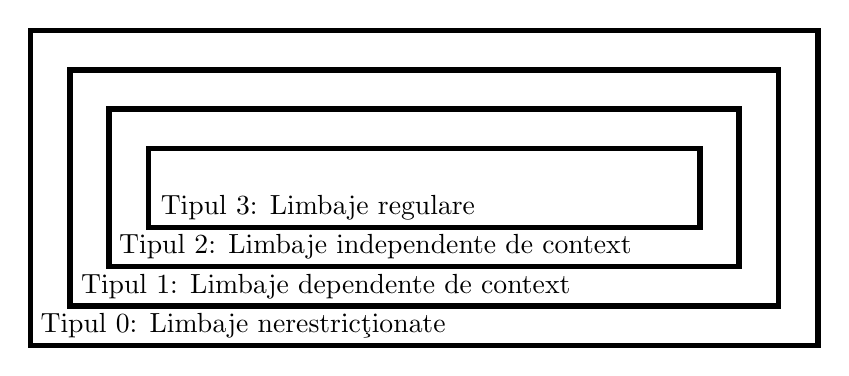
\begin{tikzpicture}
    \draw[line width=2] (0, 0) rectangle (10, 4) ;
    \draw (2.7, 0.25) node {Tipul 0: Limbaje nerestricţionate} ;
    
    \draw[line width=2] (0.5, 0.5) rectangle (9.5, 3.5);
    \draw (3.75, 0.75) node {Tipul 1: Limbaje dependente de context} ;
    
    \draw[line width=2] (1, 1) rectangle (9, 3);
    \draw (4.38, 1.25) node {Tipul 2: Limbaje independente de context} ;
    
    \draw[line width=2] (1.5, 1.5) rectangle (8.5, 2.5);
    \draw (3.65, 1.75) node {Tipul 3: Limbaje regulare} ;
\end{tikzpicture}
\end{figure}
\end{frame}



\begin{frame}{Ierarhia Chomsky}
\begin{itemize}
\item
este o ierarhie de clase de limbaje formale
\item
arată ce relaţie de incluziune există între clasele de limbaje formale
\item
fost descrisă pentru prima dată de către lingvistul Naom Chomsky, într-un articol publicat în anul 1956
\item
apartenenţa unui limbaj la unul dintre tipurile ierarhiei se determină în funcţie de forma pe care o au regulile de producţie ale unei gramatici care generează limbajul respectiv
\item
din această cauză, ierarhia Chomsky poate fi văzută şi ca o ierarhie de clase de gramatici formale
\end{itemize}
\end{frame}



\begin{frame}{Ierarhia Chomsky}
\textbf{Gramaticile de tipul 0 (gramatici nerestricționate)}
\begin{itemize}
\item
nu este impusă nicio restricţie asupra regulilor de producţie ale unei astfel de gramatici
\item
un limbaj este limbaj de tipul 0, dacă şi numai dacă el este generat de către o gramatică de tipul 0
\end{itemize}
\end{frame}



\begin{frame}{Ierarhia Chomsky}
\textbf{Gramaticile de tipul 1 (gramatici dependente de context)}
\begin{itemize}
\item
O gramatică $G = (V_{N}, \Sigma, S, P )$ se numeşte \textbf{gramatică dependentă de context} dacă şi numai dacă \textbf{toate} regulile sale de producţie au forma $\alpha A \beta \rightarrow \alpha \gamma \beta$, unde $A \in V_{N}$, $\alpha, \beta \in V^{*}$ şi $\gamma \in V^{+}$.
\item
unii autori permit şi regulile de producție de forma $S \rightarrow \epsilon$, însă cu condiţia ca $S$ să nu apară în partea dreaptă a niciunei reguli de producţie
\item
un limbaj este dependent de context, dacă şi numai dacă el este generat de către o gramatică dependentă de context
\end{itemize}
\end{frame}



\begin{frame}{Ierarhia Chomsky}
\textbf{Gramaticile de tipul 1 (gramatici dependente de context)}

Exemplu: $G = (V_{N}, \Sigma, S, P )$, unde:

\begin{itemize}
\item
$V_{N} = \{$ Propoziţie, Subiect, Atribut, Predicat, Complement, Substantiv, Verb, Adjectiv, Adverb$\}$,
\item
$\Sigma = \{$ a merge, a cânta, este, face, copilul, câinele, frumos, rău, bine, mult, ., ' '$\}$,
\item
S este Propoziţie,
\item
$P = \{$
\begin{itemize}
\item
Propoziţie $\rightarrow$ Subiect [Atribut] Predicat [Complement].,
\item
Subiect $\rightarrow$ Substantiv | Verb,
\item
Atribut $\rightarrow$ Adjectiv,
\item
Predicat $\rightarrow$ Verb,
\item
Complement $\rightarrow$ Adverb,
\item
\textbf{Verb Atribut} $\rightarrow$ a merge Atribut | a cânta Atribut,
\item
\textbf{Verb Complement} $\rightarrow$ este Complement | face Complement,
\item
Substantiv $\rightarrow$ copilul | câinele,
\item
Adjectiv $\rightarrow$ frumos | rău,
\item
Adverb $\rightarrow$ bine | mult
\end{itemize}
$\}$
\end{itemize}
\end{frame}



\begin{frame}{Ierarhia Chomsky}
\textbf{Gramaticile de tipul 2 (gramatici independente de context)}
\begin{itemize}
\item
O gramatică $G = (V_{N}, \Sigma, S, P )$ se numeşte \textbf{gramatică independentă de context} dacă şi numai dacă \textbf{toate} regulile sale de producţie au forma $A \rightarrow u$, unde $A \in V_{N}$ şi $u \in V^{*}$.
\item
un limbaj este independent de context, dacă şi numai dacă el este generat de către o gramatică independentă de context
\item
cu exceptia gramaticii de pe slide-ul anterior, toate celelalte gramatice utilizate în prezentare sunt gramatici independente de context
\end{itemize}
\end{frame}



\begin{frame}{Ierarhia Chomsky}
\textbf{Gramaticile de tipul 3 (gramatici regulare)}
\begin{itemize}
\item
O gramatică $G = (V_{N}, \Sigma, S, P )$ se numeşte \textbf{gramatică liniară dreapta} dacă este o gramatică independentă de context în care fiecare regulă de producţie este de forma $A \rightarrow a$ sau de forma $A \rightarrow aB$ sau de forma $A \rightarrow \epsilon$, unde $a \in \Sigma$, iar $A, B \in V_{N}$.
\item
O gramatică $G = (V_{N}, \Sigma, S, P )$ se numeşte \textbf{gramatică liniară stânga} dacă este o gramatică independentă de context în care fiecare regulă de producţie este de forma $A \rightarrow a$ sau de forma $A \rightarrow Ba$ sau de forma $A \rightarrow \epsilon$, unde $u \in \Sigma$, iar $A, B \in V_{N}$.
\item
O gramatică se numeşte \textbf{gramatică regulară} dacă este o gramatică liniară dreapta sau stânga.
\item
un limbaj este regular dacă şi numai dacă el este generat de către o gramatică regulară
\end{itemize}
\end{frame}



\begin{frame}{Ierarhia Chomsky}
\begin{itemize}
\item
ierarhia Chomsky arată relaţia de incluziune dintre cele patru clase de limbaje definite - prin urmare: 
\begin{itemize}
\item
orice limbaj regular este şi un limbaj independent de context
\item
orice limbaj independent de context este şi un limbaj dependent de context
\item
şi orice limbaj dependent de context este şi un limbaj nerestricţionat
\end{itemize}
\item
analog, se poate afirma că: 
\begin{itemize}
\item
nu orice limbaj nerestricţionat este şi un limbaj dependent de context
\item
nu orice limbaj dependent de context este şi limbaj independent de context
\item
nu orice limbaj independent de context este şi limbaj regular
\end{itemize}
\end{itemize}
\end{frame}



\begin{frame}{Ierarhia Chomsky}
\begin{itemize}
\item
având în vedere restricţiile impuse asupra regulilor de producţie ale fiecărui tip de gramatici formale, se observă că limbajele regulare sunt cele mai simple, iar limbajele nerestricţionate sunt cele mai complexe
\item
cu alte cuvinte, complexitatea limbajelor scade de la tipul 0 către tipul 3
\item
Exemple:
\begin{itemize}
\item
limbajele naturale sunt limbaje de tipul 0
\item
limbajele de programare sunt limbaje de tipul 2 
\item
unele aspecte ale limbajelor de programare le-ar clasifica ca şi limbaje de tipul 1, însă în practică se preferă definirea lor prin gramatici de tipul 1, adăugându-se câteva restricţii suplimentare
\item
limbajul atomilor lexicali ai unui limbaj de programare (cuvintele cheie, numele de funcţii, variabile, structuri, clase, ş.a., constantele numerice, constantele literale, constantele de tip şir de caractere, operatorii, semnele de punctuaţie) este un limbaj de tipul 3
\end{itemize}
\end{itemize}
\end{frame}



\begin{frame}{Ierarhia Chomsky}
\begin{itemize}
\item
gramaticile formale permit definirea limbajelor prin generare
\begin{itemize}
\item
pornind de la simbolul de start, prin derivări succesive, putem genera orice propoziţie a limbajului 
\end{itemize}
\item
cum se poate rezolva problema inversă? 
\begin{itemize}
\item
fiind dată o propoziţie oarecare, cum se poate stabili dacă ea aparţine unui anumit limbaj (definit de o gramatică dată)?
\item
pentru aceasta se foloseşte un "dispozitiv" capabil sa recunoască dacă o propoziţie dată aparţine sau nu limbajului pe care el îl defineşte
\end{itemize}
\end{itemize}
\end{frame}



\begin{frame}{Ierarhia Chomsky}
Tipuri de "dispozitive" necesare stabilirii faptului că o propoziție dată aparține sau nu unui limbaj dat, în funcție de complexitatea acestuia\\

\begin{figure}
\begin{tabular}{ l | c | r | } 
\hline 
\textbf{Gramatici de tipul 3} & \textbf{automate finite} \\ 
\textbf{Gramatici de tipul 2} & \textbf{automate finite cu memorie (stivă)} \\ 
Gramatici de tipul 1 & mașină Turing cu bandă limitată \\ 
Gramatici de tipul 0 & mașină Turing \\ 
\hline 
\end{tabular}
\end{figure}
\end{frame}



\begin{frame}{Arbori de analiză gramaticală}
\begin{itemize}
\item
Definiții: graf orientat, arbore, arbore sintactic
\item
Arbori sintactici descendenți
\item
Arbori sintactici ascendenți
\item
Analiza gramaticală
\end{itemize}
\end{frame}



\begin{frame}{Arbori de analiză gramaticală}
\begin{itemize}
\item
Fie $M$ o mulţime de noduri şi $R$ o relaţie binară peste M. Atunci $G=(M, R)$ se numeşte \textbf{graf orientat}. 
\item
Dacă $(a, b) \in R$, atunci definim următoarele mulţimi:
\begin{itemize}
\item
$input(a) = \{ b | (b, a) \in R \}$,
\item
$output(a) = \{ b | (a, b) \in R \}$.
\end{itemize}
\item
\textbf{Un arbore} este un graf orientat $(M, R)$ cu următoarele restricţii:
\begin{itemize}
\item
$\exists \; r \in M$ unic, astfel încât $input(r) = \emptyset$,
\item
$\forall \; a \in M, \; a \neq r, \; card(input(a)) = 1$,
\item
$\forall \; a \in M, \; (r, a) \in R^{*}$.
\end{itemize}
\end{itemize}
\end{frame}



\begin{frame}{Arbori de analiză gramaticală}
Fie o gramatică formală $G = (V_{N}, \Sigma, S, P )$. Un \textbf{arbore de derivare} (arbore sintactic) $A=(M, R)$ este un arbore etichetat ordonat de la stânga la dreapta cu proprietăţile:
\begin{enumerate}
\item
rădăcina arborelui este etichetată cu $S$,
\item
pentru orice nod $a \in M$ cu descendenţi, astfel încât A este eticheta nodului $a$, iar $X_{1}, X_{2}, \dots, X_{i}$ sunt etichetele descendenţilor lui a, $\exists \; A \rightarrow X_{1} X_{2} \dots X_{i} \in P$.
\end{enumerate}
\end{frame}



\begin{frame}{Arbori de analiză gramaticală}
\begin{itemize}
\item
arborii sintactici sunt o reprezentare arborescentă a succesiunii de derivări prin care se generează o anumită propoziţie
\item
fiecare nod al arborelui care nu este frunză, este etichetat cu un neterminal
\item
fiecare frunză a arborelui este etichetată cu un terminal
\item
citind etichetele nodurilor arborelui (de la stânga la dreapta) de pe un nivel dat se obţine o formă propoziţională
\end{itemize}
\end{frame}



\begin{frame}{Arbori de analiză gramaticală}
\begin{itemize}
\item
construcţia arborelui sintactic pentru o propoziţie dată se poate face în două moduri:
\begin{itemize}
\item
se poate porni de la rădăcină către frunze, adică de la simbolul de start către propoziţie

(construcţie descendentă - \textbf{arbore sintactic descendent})
\item
se poate porni de la frunze către rădăcină, adică de la propoziţie către simbolul de start

(construcţie ascendentă - \textbf{arbore sintactic ascendent})
\end{itemize}
\item
evident, arborele sintactic descendent al unei propoziţii este identic cu arborele sintactic ascendent al aceleiaşi propoziţii
\end{itemize}
\end{frame}



\begin{frame}{Arbori de analiză gramaticală}
\begin{itemize}
\item
arborele sintactic \textbf{descendent} corespunzător propoziţiei \textit{Ana învaţă.} și gramaticii prezentate anterior:

\begin{figure}[H]
\centering
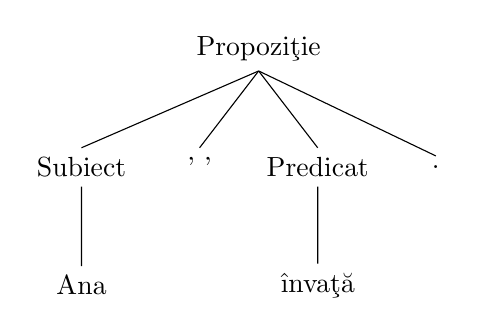
\begin{tikzpicture}
\node {Propoziţie}
child {node {Subiect} 
   child {node {Ana}}
}
child {node {' '}}
child {node {Predicat}
   child {node {învaţă}}
}
child {node {.}
};
\end{tikzpicture}
\end{figure}
\end{itemize}
\end{frame}



\begin{frame}{Arbori de analiză gramaticală}
\begin{itemize}
\item
arborele sintactic \textbf{ascendent} corespunzător propoziţiei \textit{Ana învaţă.} și gramaticii prezentate anterior:

\begin{figure}[H]
\centering
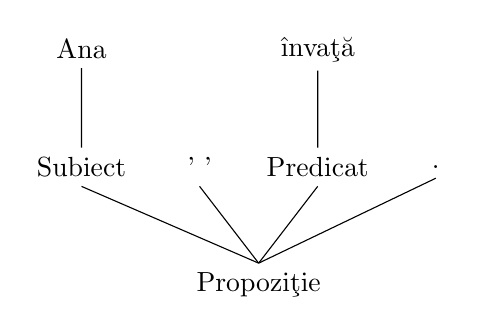
\begin{tikzpicture}
\node {Propoziţie}[grow=up]
child {node {.}}
child {node {Predicat}
   child {node {învaţă}}
}
child {node {' '}}
child {node {Subiect} 
   child {node {Ana}}
};
\end{tikzpicture}
\end{figure}
\end{itemize}
\end{frame}



\begin{frame}{Arbori de analiză gramaticală}
\begin{itemize}
\item
verificarea dacă o propoziţie dată aparţine limbajului definit de o gramatică formală se numeşte \textbf{analiză sintactică}
\item
ea constă în încercarea de a construi arborele sintactic al propoziţiei date, conform gramaticii care defineşte limbajul respectiv
\begin{itemize}
\item
dacă se poate construi un arbore sintactic - propoziția aparţine limbajului
\item
dacă nu se poate construi un arbore - propoziţia nu aparţine limbajului
\end{itemize}
\item
clasificare
\begin{itemize}
\item
\textbf{analiză sintactică descendentă} - încearcă construirea arborelui sintactic în sens descendent
\item
\textbf{analiză sintactică ascendentă} - încearcă construirea arborelui în sens ascendent
\end{itemize}
\end{itemize}
\end{frame}



\begin{frame}{Intrebari recapitulative}
\begin{itemize}
\item
Fie $G = (V_{N}, \Sigma, S, P )$ , astfel încât $card(\Sigma)=m$, iar $card(V_{N})=n$. Care ar trebui să fie valoarea minimă pentru $card(P)$ astfel încât definiția gramaticii să fie corectă? Explicați.
\newline 

\item
Având în vedere mulțimile $V_0$, $V_1$, \dots, $V_i$ folosite în definiția mulțimii V*, să se scrie cine este $V_{i+1} \setminus V_i$ și să se explice.
\newline 

\item
Care este restricția impusă numărului de elemente ale mulțimii terminalelor din definiția unei gramatici, așa cum a fost introdusă la curs?

\end{itemize}
\end{frame}



\begin{frame}{Intrebari recapitulative}
\begin{itemize}
\item
Fie $G = (V_{N}, \Sigma, S, P )$ , astfel încât $card(\Sigma)=m$,  $card(VN)=n$, iar $card(P)=k$ și fie $p$ un element din mulțimea $L(G)$. Câte frunze va avea arborele sintactic corespunzător lui p?
\newline 

\item
Prezentați care sunt asemănările dintre o formă propozițională și o propoziție.
\newline

\item
Prezentați felul în care o gramatică $G$ definește semantica unui limbaj.
\newline

\end{itemize}
\end{frame}



\begin{frame}{Intrebari recapitulative}
\begin{itemize}

\item
Care este relația dintre alfabetul unei gramatici și alfabetul limbajului definit de către gramatica respectivă?
\newline

\item
Explicați care este diferența dintre relația de derivare directă și relația de derivare în k pași.
\newline

\item
Enumerați situațiile în care relația de derivare în k pași este o relație între forme propoziționale.

\end{itemize}
\end{frame}



\begin{frame}{Intrebari recapitulative}
\begin{itemize}

\item
Explicați cauza diferențelor dintre derivarea stângă și derivarea dreapta pentru o propoziție care aparține unui limbaj regular, definit de o gramatică regulară.
\newline

\item
Pornind de la definiția formelor propoziționale, explicați de ce simbolul de start al unei gramatici este o formă propozițională.

\end{itemize}
\end{frame}



\begin{frame}{Intrebari recapitulative}
\begin{itemize}

\item
Explicați semantica ierarhiei Chomsky.
\newline

\item
Câți arbori de derivare pot fi construiți pentru o propoziție dată, pe baza unei gramatici care definește limbajul căreia îi aparține propoziția? Explicați.
\newline

\end{itemize}
\end{frame}



\begin{frame}{Intrebari recapitulative}
\begin{itemize}

\item
Fie următoarele două succesiuni de relații de derivare realizate pe baza unei gramatici $G$ date, pentru o propoziție $p \in L(G)$:

\begin{enumerate}
\item
succesiunea de relații de derivare bazate pe derivare dreapta,
\item
succesiunea de relații de derivare bazate pe derivarea stânga.
\end{enumerate}

Scrieți care este numărul minim de forme propoziționale comune celor două succesiuni de relații de derivare și explicați.
\newline

\item
Fie $G$ o gramatică. Se notează cu $F(G)$ mulțimea formelor propoziționale care se pot defini pe baza gramaticii $G$. Scrieți ce relație există între $F(G)$ și $L(G)$ și explicați.

\end{itemize}
\end{frame}



%%%%%%%%%%%%%%%%%%%%%%%%%%%%%%%%%%%%%%%%%%%%%%%%%%%%%%%%%%



\begin{frame}{Limbaje regulare}
\textbf{Cuprins}
\begin{itemize}
\item
Automate cu stări finite
\item
Expresii regulare
\end{itemize}
\end{frame}



\begin{frame}{Automate cu stări finite}
\textbf{Cuprins}
\begin{itemize}
\item
Automate finite deterministe
\item
Automate finite nedeterministe
\item
Automate finite $\epsilon$
\item
Automate finite vs. Gramatici formale
\end{itemize}
\end{frame}



\begin{frame}{Automate cu stări finite}
\begin{itemize}
\item
reprezintă un model matematic care permite descrierea proceselor de calcul
\item
un automat finit este gândit ca şi o maşină abstractă, care, la un moment dat, se poate afla într-o singură stare, dintr-o mulţime finită de stări date
\item
starea în care se află automatul la un moment dat se numeşte \textbf{stare curentă}
\item
starea în care se află automatul înainte de începerea procesului de calcul se numeşte \textbf{stare iniţială}
\item
automatul poate să treacă dintr-o stare în alta în funcţie de anumite intrări
\item
schimbarea stării curente a automatului (trecerea din starea curentă într-o altă stare, care devine noua stare curentă) se numeşte \textbf{tranziţie}
\end{itemize}
\end{frame}



\begin{frame}{Automate cu stări finite}
\textbf{Clasificare}
\begin{itemize}
\item
dacă pentru o stare curentă şi pentru o intrare dată automatul poate să facă o singură tranziţie (există o singură stare în care poate să treacă, în baza intrării date), atunci el este un \textbf{automat finit determinist}
\item
dacă pentru o stare curentă şi o intrare dată un automat poate efectua mai multe tranziţii (există mai multe stări în care poate să treacă, în baza intrării date), atunci el este un \textbf{automat finit nedeterminist}
\end{itemize}
\end{frame}



\begin{frame}{Automate cu stări finite}
\begin{itemize}
\item
în teoria limbajelor formale, automatele finite sunt utilizate pentru a defini sau pentru a recunoaşte \textbf{limbaje regulare}
\item
cu alte cuvinte, expresivitatea unui anumit finit este aceeaşi cu cea a unei gramatici regulare
\item
intrarea pe baza căreia se realizează tranziţiile este dată de către următorul simbol neanalizat din şirul de la intrare
\item
mulţimea şirurilor de simboluri pe care le recunoaşte un automat finit dat, se numeşte limbajul definit de către automat
\item
automatele finite sunt utilizate pentru a verifica dacă o propoziţie dată aparţine sau nu unui anumit limbaj regular, adică dacă este o propoziţie corectă din punctul de vedere al limbajului regular avut în vedere
\end{itemize}
\end{frame}



\begin{frame}{Automate finite deterministe}
Un \textbf{automat finit determinist} este un cvintuplu $AFD=(\Sigma, Q, F, q_{0}, f)$, în care:
\begin{itemize}
\item
$\Sigma$ este o mulţime finită de simboluri şi se numeşte alfabetul limbajului de intrare al automatului;
\item
$Q$ este mulţimea finită de stări ale automatului;
\item
$F$ este mulţimea stărilor finale ale automatului, $F \subseteq Q$;
\item
$q_{0}$ este starea iniţială a automatului, $q_{0} \in Q$;
\item
$f$ este funcţia de tranziţie, $f:Q \times \Sigma \rightarrow Q$.
\end{itemize}
\end{frame}



\begin{frame}{Automate finite deterministe}
\textbf{Reprezentare}
\begin{itemize}
\item
prin graful de tranziţie
\begin{itemize}
\item
\textbf{stările} se reprezintă prin cercuri, care au înscrise în ele numele
\item
\textbf{starea iniţială} este marcată printr-o săgeată
\item
\textbf{stările finale} sunt marcate prin dublarea cercurilor
\item
\textbf{tranziţiile} sunt reprezentate prin săgeţi între stări, deasupra cărora se scrie simbolul/simbolurile de la intrare în baza cărora se face schimbarea stării
\end{itemize}
\item
prin tabela de tranziţie
\begin{itemize}
\item
stările finale se marchează printr-o steluţă
\end{itemize}
\end{itemize}
\end{frame}



\begin{frame}{Automate finite deterministe}
\textbf{Exemplu}
\begin{itemize}
\item
Fie automatul finit determinist $AFD=(\Sigma, Q, F, q_{0}, f)$, unde:

\begin{itemize}
\item
$\Sigma = \{ 0, 1 \}$,
\item
$Q = \{ q_{0}, q_{1}, q_{2} \}$,
\item
$F=\{ q_{0}, q_{2} \}$
\item
starea iniţială este $q_{0}$,
\item
iar funcţia de tranziţie $f$ se deduce din graful de tranziţie, sau respectiv din tabelul de tranziţie.
\end{itemize}
\item
care acceptă limbajul următor:

$L(AFD) = \{ 0^{n}1^{m}0 | n \geq 0, \; m \geq 1 \}$, 

unde am notat cu $a^{t}$ concatenarea simbolului $a$ cu el însuşi de un număr de $t$ ori
\end{itemize}
\end{frame}



\begin{frame}{Automate finite deterministe}
\begin{figure}[H]
\centering
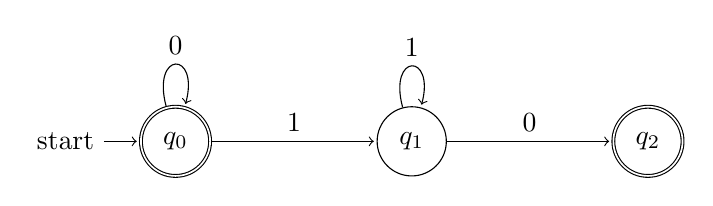
\begin{tikzpicture}[shorten >=1pt,node distance=3cm,on grid,auto]

  \node[state,initial,accepting]	(0)              		{$q_0$};
  \node[state]    			(1)   [right  of=0] 	{$q_1$};
  \node[state,accepting]              (2)  [right of=1] 	{$q_2$};   

 \path[->]
     (0)	edge [loop above]	node	{0} ()
           edge			node	{1} (1)
     (1)	edge			node	{0} (2)
           edge	[loop above] node	{1} (1)

%         (1)  edge    [bend right]         node [below]{b}    (13)
%     (123)  edge                                node             {b}    ()
%               edge                                 node             {a}    (03)
%      (03)  edge    [bend left]            node             {a}    (013)
%               edge    [bend right]         node [above]{b}    (123)
%     (013) edge    [loop below]         node              {a}    ()
%               edge                                 node             {b}    (123)
%     (13)   edge    [bend right=70]    node [below]{a}    (03)
%               edge                                 node              {b}    (123)
  ;
\end{tikzpicture}
\caption{Graful de tranziţie}
\end{figure}

\begin{figure}[H]
\centering
\begin{tabular}{ l | c r }
      $\;\;f$     &            0 &            1\\
   \hline
  *$q_{0}$    & $q_{0}$ & $q_{1}$\\
  $\;\;q_{1}$ & $q_{2}$ & $q_{1}$\\
  *$q_{2}$    &            -  &             -\\
\end{tabular}
\caption{Tabela de tranziţie}
\end{figure}
\end{frame}



\begin{frame}{Automate finite deterministe}
\begin{itemize}
\item
un automat citeşte un şir finit de simboluri 

$a_{1} a_{2} \dots a_{n}$, $a_{i} \in \Sigma, \forall \; 1 \leq i \leq n$

\item
în funcţie de fiecare simbolul citit şi de starea curentă în care se află automatul la citirea simbolului respectiv, acesta execută o tranziţie, în conformitate cu definiţia funcţiei de tranziţie
\item
automatul se opreşte 
\begin{itemize}
\item
după ce a citit toate simbolurile din propoziţia de intrare
\item
sau atunci când pentru simbolul următor de la intrare şi pentru starea curentă în care se află, nu se poate executa nicio tranziţie
\end{itemize}
\end{itemize}
\end{frame}



\begin{frame}{Automate finite deterministe}
\begin{itemize}
\item
Fie $AFD=(\Sigma, Q, F, q_{0}, f)$ un automat finit. O pereche 

$(x, \; q), x \in \Sigma^{*}, \; q \in Q$ 

se numeşte \textbf{configuraţie} a automatului finit. 
\item
$q$ este starea curentă a automatului, 
\item
iar $x$ este restul şirului de la intrarea automatului, care nu a fost încă analizat
\end{itemize}
\end{frame}



\begin{frame}{Automate finite deterministe}
\begin{itemize}
\item
Fie $AFD=(\Sigma, Q, F, q_{0}, f)$ un automat finit. \textbf{Relaţia de mişcare} este o relaţie binară notată cu 

$\vdash$ $(\vdash \subseteq (\Sigma^{*} \times Q) \times (\Sigma^{*} \times Q))$ 

şi definită astfel:

$(ax, q) \vdash (x, q') \Leftrightarrow f(q, a) = q'$, 

unde $a \in \Sigma$, $x \in \Sigma^{*}$, $q, q' \in Q$.

\item
De exemplu:

$(00, q_0) \vdash (0, q_0)$
\end{itemize}
\end{frame}



\begin{frame}{Automate finite deterministe}
\begin{itemize}
\item
Fie $AFD=(\Sigma, Q, F, q_{0}, f)$ un automat finit. \textbf{Relaţia de mişcare în k paşi} este o relaţie binară notată cu 

$\vdash^{k}$ $(\vdash^{k} \subseteq (\Sigma^{*} \times Q) \times (\Sigma^{*} \times Q))$ 

şi definită astfel:

$(a_{1} a_{2} \dots a_{k} x, q) \vdash^{k} (x, q') \Leftrightarrow \exists \; k+1$ configuraţii astfel încât 

$(a_{i}a_{i+1} \dots a_{k}x, q_{i}) \vdash (a_{i+1} \dots a_{k}x, q_{i+1}), \; \forall \; 1 \leq i \leq k$, $q = q_{1}, q' = q_{k+1}$, 

unde $a_{1}, a_{2}, \dots, a_{k} \in \Sigma, \; x \in \Sigma^{*}, \; q, q', q_{1}, q_{2}, \dots, q_{k+1} \in Q$.

\item
De exemplu:

$(0001, q_0) \vdash^3 (1, q_0)$
\end{itemize}
\end{frame}



\begin{frame}{Automate finite deterministe}
\begin{itemize}
\item
Fie $AFD=(\Sigma, Q, F, q_{0}, f)$ un automat finit. \textbf{Relaţia generală de mişcare} este o relaţie binară notată cu 

$\vdash^{*}$ $(\vdash^{*} \subseteq (\Sigma^{*} \times Q) \times (\Sigma^{*} \times Q))$ 

şi definită astfel:

$(x_{1}, q) \vdash^{*} (x_{2}, q') \Leftrightarrow (x_{1} = x_{2}$ şi $q = q')$ sau $((x_{1}, q) \vdash^{+} (x_{2}, q'))$, 

unde $x_{1}, x_{2} \in \Sigma^{*}, q, q' \in Q$.
\end{itemize}
\end{frame}



\begin{frame}{Automate finite deterministe}
\begin{itemize}
\item
Fie $AFD=(\Sigma, Q, F, q_{0}, f)$ un automat finit. Se spune că $x \in \Sigma^{*}$ este o \textbf{propoziţie acceptată} de către automat, dacă există următoarea relaţie de mişcare: 

$(x, q_{0}) \vdash^* (\epsilon, q')$, unde $q' \in F$.
\item
o propoziţie acceptată de către un automat finit AFD este orice şir de simboluri din $\Sigma$, care, citit simbol cu simbol de la stânga spre dreapta, duce automatul din starea iniţială într-o stare finală
\end{itemize}
\end{frame}



\begin{frame}{Automate finite deterministe}
\begin{itemize}
\item
Fie $AFD=(\Sigma, Q, F, q_{0}, f)$ un automat finit. \textbf{Limbajul acceptat} de către automatul AFD se notează cu $L(AFD)$ şi est definit în felul următor:

$L(AFD) = \{ x \in \Sigma^{*} | f^{*}(q_{0}, x) \in F \}$,

unde $f$ este extinsă la $f^{*}$ astfel:
\begin{itemize}
\item
$f^{*}(q, \epsilon) = q$,
\item
$f^{*}(q, ax) = f^{*}(f(q, a), x)$.
\end{itemize}
\item
cu alte cuvinte, limbajul acceptat de către un automat finit AFD este mulţimea formată din toate şirurile de simboluri peste $\Sigma$ care sunt acceptate de către automat
\end{itemize}
\end{frame}



\begin{frame}{Automate finite deterministe}
\begin{itemize}
\item
automatele finite au un număr fix şi limitat de stări
\item
există limbaje care nu pot fi recunoscute de către un astfel de automat finit - evident este vorba de limbajele care nu sunt regulare
\item
limbajul $L=\{a^n b a^n | n > 0 \}$
\begin{itemize}
\item
un automat finit determinist ar trebui să se afle într-o stare diferită după citirea şirului $a^k$, pentru fiecare valoare a lui $k>0$ (deoarece numai după k citiri de a, automatul trebuie să accepte şirul $b a^k$)
\item
rezultă necesitatea unui număr infinit de stări, ceea nu este posibil
\end{itemize}
\end{itemize}
\end{frame}



\begin{frame}{Automate finite nedeterministe}
\begin{itemize}
\item
Un \textbf{automat finit nedeterminist} este un cvintet $AFN=(\Sigma, Q, F, q_{0}, f)$, unde $\Sigma, Q, F, q_{0}$ sunt definite în acelaşi mod ca şi pentru un automat finit determinist, iar funcţia de tranziţie $f$ este definită astfel:

$f:Q \times \Sigma \rightarrow 2^{Q} - \emptyset$,

unde prin $2^{Q}$ s-a notat mulțimea tuturor submulțimilor mulțimii $Q$.
\item
pentru o aceeaşi stare şi pentru un acelaşi simbol de la intrare, pot exista mai multe tranziţii posibile, ceea ce înseamnă că automatul poate trece în mai multe stări
\item
evident, automatul nu are niciun criteriu suplimentar în baza căruia să facă alegerea.
\end{itemize}
\end{frame}



\begin{frame}{Automate finite nedeterministe}
\begin{itemize}
\item
Fie automatul finit $M=(\Sigma, Q, F, q_{0}, f)$, unde:
\begin{itemize}
\item
$\Sigma=\{ 0, 1 \}$
\item
$Q=\{ q_{0}, q_{1}, q_{2}, q_{3} \}$
\item
$F=\{ q_{3} \}$
\item
iar funcţia de tranziţie $f$ este definită prin următorul graf de tranziţie:
\end{itemize}

\begin{figure}[H]
\centering
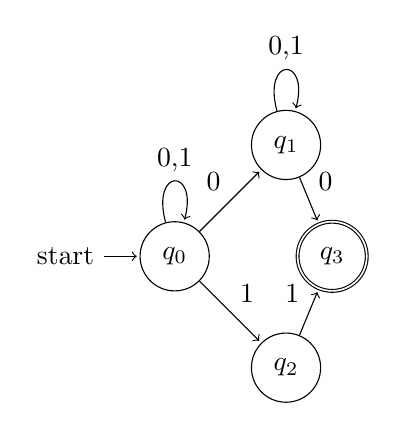
\begin{tikzpicture}[shorten >=1pt,node distance=2cm,on grid,auto]

  \node[state,initial]			(0)              			{$q_0$};
  \node[state]    			(1)   [above right  of=0] 	{$q_1$};
  \node[state]    			(2)   [below right  of=0] 	{$q_2$};
  \node[state,accepting]              (3)   [right of=0] 		{$q_3$};   

 \path[->]
     (0)	edge 			node	{0} (1)
           edge			node	{1} (2)
           edge	[loop above]	node	{0,1} (0)
     (1) edge			node	{0} (3)
           edge [loop above]	node	{0,1} (1)
     (2)	edge			node	{1} (3)
  ;
\end{tikzpicture}
\end{figure}
\end{itemize}
\end{frame}



\begin{frame}{Automate finite nedeterministe}
\begin{itemize}
\item
Pentru orice automat finit nedeterminist $M=(\Sigma, Q, F, q_{0}, f)$, există un automat finit determinist $M'$ echivalent, adică $L(M') = L(M).$
\item
Fie $M=(\Sigma, Q, F, q_{0}, f)$ un automat finit nedeterminist. Atunci automatul finit determinist echivalent $M'$ este definit astfel:

$M'=(\Sigma, Q', F', q_{0}', f')$, 

unde:
\end{itemize}
\end{frame}



\begin{frame}{Automate finite nedeterministe}
\begin{center}
\resizebox{\columnwidth}{!}{%
  \begin{tabular}{| l | l | p{5cm} | }
    \hline
    & AFN & AFD \\ \hline
    Alfabetul & $ \Sigma $ & $ \Sigma $\\ \hline
    M. stărilor & $Q=\{q_{0}, q_{1}, q_{2}, \dots q_{n}\}$ & $Q'=\{ \emptyset, \{q_{0}\}, \{q_{1}\}, \{q_{2}\}, \linebreak \dots, \{q_{n}\}, \{q_{0}, q_{1}\}, \{q_{0}, q_{2}\}, \dots, \linebreak \{q_{0}, q_{n}\}, \dots, \{q_{n-1}, q_{n}\}, \dots, \linebreak \{q_{0}, q_{1}, \dots q_{n}\} \}$ \\ \hline
    Starea iniţială & $q_{0}$ & $\{q_{0}$\} \\ \hline
    M. stărilor finale & $F \subset Q$ & $F'=\{s \in Q'| \linebreak s$ \textit{conţine cel puţin o stare finală  a AFN} $\}$ \\ \hline
    Tranziţii & f & $f'(\{ q_{i_{1}}, q_{i_{2}}, \dots, q_{i_{k}} \}, a)= \linebreak f(q_{i_{1}}, a) \cup f(q_{i_{2}}, a) \cup \dots \cup f(q_{i_{k}}, a)$ \\ \hline
  \end{tabular}%
}
\end{center}
\end{frame}



\begin{frame}{Automate finite nedeterministe}
După generarea elementelor automatului finit determinist pornind de la cele ale automatului finit nedeterminist, se elimina stările şi tranziţiile inutile:
\begin{itemize}
\item
stările inutile sunt stările la care automatul nu poate ajunge pornind din starea iniţială şi făcând una sau mai multe tranziţii
\item
tranziţiile inutile sunt tranziţiile care pleacă dintr-o stare inutilă
\end{itemize}
\end{frame}



\begin{frame}{Automate finite nedeterministe}

\begin{figure}
\textbf{AFN:}

\centering
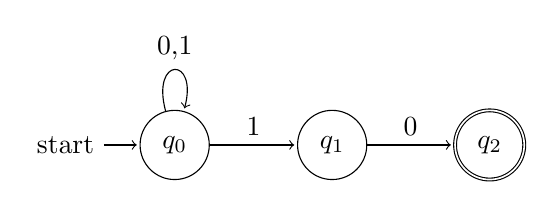
\begin{tikzpicture}[shorten >=1pt,node distance=2cm,on grid,auto]
  \node[state,initial]	(0)              		{$q_0$};
  \node[state]    			(1)   [right  of=0] 	{$q_1$};
  \node[state,accepting]              (2)  [right of=1] 	{$q_2$};   

 \path[->]
     (0)	edge [loop above]	node	{0,1} ()
           edge			node	{1} (1)
     (1)	edge			node	{0} (2)
  ;
\end{tikzpicture}
\end{figure}
\end{frame}



\begin{frame}{Automate finite nedeterministe}
\begin{figure}
\textbf{AFD echivalent (complet - inclusiv stările și tranzițiile inutile):}

\centering
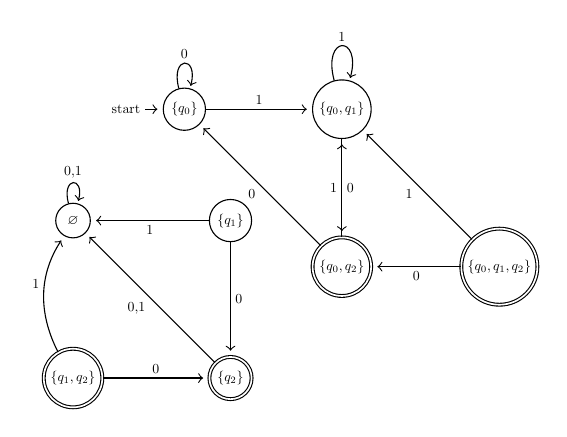
\begin{tikzpicture}[scale=.5, transform shape,shorten >=2pt,node distance=4cm,on grid,auto]
  \node[state,initial]	(0)              		{$\{q_0\}$};
  \node[state]    			(1)   [right  of=0] 	{$\{q_0,q_1\}$};  
  \node[state,accepting]    	(2)   [below  of=1] 	{$\{q_0,q_2\}$};
  \node[state,accepting]    	(3)   [right  of=2] 	{$\{q_0,q_1,q_2\}$};
  \node[state ]                              (4)  [below left of=0] 	{$\varnothing$}; 
  \node[state]    			(5)   [right  of=4] 	{$\{q_1\}$};
  \node[state,accepting]          	(6)  [below of=5] 	{$\{q_2\}$}; 
  \node[state,accepting]		(7)   [left  of=6] 	{$\{q_1,q_2\}$};

 \path[->]
     (0)	edge [loop above]	node	{0} (0)
     (1) edge [loop above]   node	{1} (1)
     (0) edge                         node  {1} (1)
     (3)	edge                         node  {0} (2)
     (3)	edge                         node  {1} (1)
     (2)	edge                         node  {1} (1)
     (1)	edge                         node  {0} (2)
     (2)	edge                         node  {0} (0)
  (5)	edge                         node  {1} (4)
  (5)	edge                         node  {0} (6)
  (6)	edge                         node  {0,1} (4)
  (7)	edge                         node  {0} (6)
  (7)	edge  [bend left]                       node  {1} (4)
     (4) edge [loop above]   node	{0,1} (4)
  ;
\end{tikzpicture}
\end{figure}
\end{frame}



\begin{frame}{Automate finite nedeterministe}
\begin{figure}
\textbf{AFD echivalent (după eliminarea stărilor și tranzițiilor inutile):}

\centering
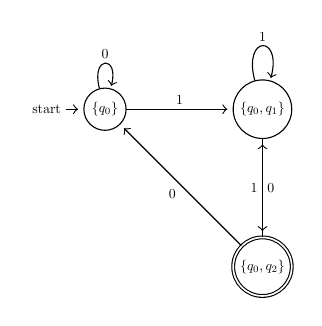
\begin{tikzpicture}[scale=.5, transform shape,shorten >=2pt,node distance=4cm,on grid,auto]
  \node[state,initial]	(0)              		{$\{q_0\}$};
  \node[state]    			(1)   [right  of=0] 	{$\{q_0,q_1\}$};  
  \node[state,accepting]    	(2)   [below  of=1] 	{$\{q_0,q_2\}$};

 \path[->]
     (0)	edge [loop above]	node	{0} (0)
     (1) edge [loop above]   node	{1} (1)
     (0) edge                         node  {1} (1)
     (2)	edge                         node  {1} (1)
     (1)	edge                         node  {0} (2)
     (2)	edge                         node  {0} (0)
  ;
\end{tikzpicture}
\end{figure}
\end{frame}



\begin{frame}{Automate finite $\epsilon$}
\begin {itemize}
\item
O tranziţie $\varepsilon$ este o tranziţie dintr-o stare în alta,
fără a “consuma” niciun simbol din şirul de intrare.
\item
Aceste tranziţii sunt practic tranziţii spontane, care se fac fără a privi la simbolul care urmează în şirul de intrare.
\end{itemize}

\begin{figure}[H]
\centering
\begin{tikzpicture}[->,>=stealth',shorten >=1pt,auto,node distance=3cm, on grid,auto]
  \node[initial,draw, circle] (A)                    {};
 
  \node[accepting,draw, circle]         (D) [below right of=A] {};
  \node[draw, circle]         (B) [right of=A] {};
  \node[accepting,draw, circle]         (C) [above right of=D] {};
  
  \path (A) edge              node [below]{+ | -} (B)
 	    edge [bend left=50] node {$\varepsilon$} (B)
   	    edge	    node[left] {0} (D)
          (B) edge                node {1|2|...|9} (C)
          (C) edge  [loop right]            node {0|1|...|9} (C);					
\end{tikzpicture}
\end{figure}
\end{frame}

\begin{frame}{Automate finite $\epsilon$}
\begin{itemize}
\item
Orice AFN este de fapt un AF-$\epsilon$ care nu are nicio tranziţie $\epsilon$.
\item
AFN şi AF- $\epsilon$ sunt echivalente.
\item
Deducerea AFN echivalent unui AF- $\epsilon$ constă în construirea unui AFN care accepta acelaşi limbaj ca şi AF- $\epsilon$ de la care am pornit.
\item
Construirea se face combinând fiecare tranziţie $\epsilon$ cu următoarea tranziţie care se face pe baza simbolului de la intrare.
\end{itemize}
\end{frame}



\begin{frame}{Automate finite $\epsilon$}
\begin{itemize}
\item
Pentru orice automat finit $\epsilon$ $M=(\Sigma \cup \{ \epsilon \}, Q, F, q_{0}, f)$, există un automat finit nedeterminist $M'$ echivalent, adică $L(M') = L(M).$

\item
Fie $M=(\Sigma \cup \{ \epsilon \}, Q, F, q_{0}, f)$ un automat finit $\epsilon$. Atunci automatul finit nedeterminist echivalent $M'$ este definit astfel $M'=(\Sigma, Q', F', q_{0}, f')$, unde:

\begin{center}
\resizebox{\columnwidth}{!}{%
  \begin{tabular}{| l | l | p{8cm} | }
    \hline
    & AF$\epsilon$ & AFN \\ \hline
    Alfabetul & $ \Sigma \cup \{ \epsilon \} $ & $ \Sigma $\\ \hline
    M. stărilor & $Q=\{q_{0}, q_{1}, q_{2}, \dots q_{n}\}$ & $Q'=\{q_{0}, q_{1}, q_{2}, \dots q_{n}\}$ \\ \hline
    Starea iniţială & $q_{0}$ & $q_{0}$\\ \hline
    M. stărilor finale & $F \subset Q$ & $F'=F \cup \{q' \in Q' \; | \; \exists \; s \in CL(q')|_{AF\epsilon} \; a.i. \; s \in F \}$ \\ \hline
    Tranziţii & f & $f'(q,a)=f(q,a)$ \newline $ f'(q,b) = f(f( \dots f(q,\epsilon)\dots,\epsilon),b) $ \newline $ \; \forall \; q \in Q' \; şi \; a,b \in \Sigma $ \\ \hline
  \end{tabular}%
}
\end{center}
\end{itemize}
\end{frame}



\begin{frame}{Automate finite $\epsilon$}
\begin{itemize}
\item Tranziţia $\epsilon$ duce din starea iniţiala în starea a doua.
\item Din starea a doua se trece în starea a treia pe baza $1\mid2\mid\dots\mid9$.
\item Înlocuim tranziţia $\epsilon$ (cea în roşu) cu o tranziţie din starea iniţială direct în starea a treia pe baza $1\mid2\mid\dots\mid9$ (cea în albastru).
\end{itemize}

\begin{figure}[H]
\centering
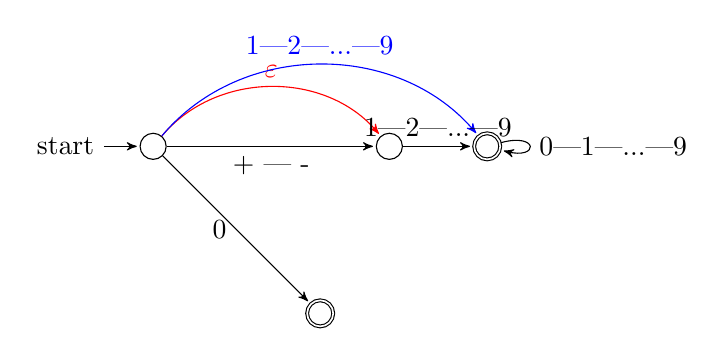
\begin{tikzpicture}[->,>=stealth',shorten >=1pt,auto,node distance=3cm, on grid,auto]
  \node[initial,draw, circle] (A)                    {};
 
  \node[accepting,draw, circle]         (D) [below right of=A] {};
  \node[draw, circle]         (B) [right of=A] {};
  \node[accepting,draw, circle]         (C) [above right of=D] {};
  
  \path (A) edge                         node [below]{+ | -} (B)
 	       edge [bend left=50, red] node {$\varepsilon$} (B)
       	       edge [bend left=50, blue] node {1|2|...|9} (C)
   	       edge	                   node[left] {0} (D)
            (B) edge                         node {1|2|...|9} (C)
            (C) edge  [loop right]     node {0|1|...|9} (C);					
\end{tikzpicture}
\end{figure}
\end{frame}



\begin{frame}{Automate finite $\epsilon$}
\begin{itemize}
\item
După eliminarea tranziţiilor $\epsilon$, toate stările ale căror închideri conţin o stare finală, devin stări finale.
\item
Dacă starea în care se trece prin tranziţia $\epsilon$ nu are nicio tranziţie pe baza intrării, atunci:
\begin{itemize}
	\item
	Dacă starea respectivă este stare finală, starea din care pleacă tranziţia $\epsilon$ devine stare finală, iar tranziţia $\epsilon$ este eliminată.
	\item
	Altfel, se elimină pur şi simplu tranziţia $\epsilon$ (fiind oricum o tranziţie inutilă).
\end{itemize}
\end{itemize}
\end{frame}



\begin{frame}{Automate finite $\epsilon$}
\begin{itemize}
\item
Fie $AF-\epsilon=(\Sigma \cup \{ \epsilon \}, Q, F, q_{0}, f)$ un automat finit $ \epsilon $. \textbf{Închiderea unei stări (closure)} $q \in Q$, notată cu $CL(q)$, este mulţimea tuturor stărilor la care se poate ajunge pornind din starea $ q $ şi făcând numai tranziţii $\epsilon$:

$CL(q) = \{ q' \in Q \; | \; (x, q) \vdash^+ (x, q') \}$.
\item
Pentru a specifica faptul că închiderea unei stări $ q $ se calculează pentru un anumit automat finit $ AF $, vom folosi notaţia $ CL(q)|_{AF} $.
\end{itemize}
\end{frame}



\begin{frame}{Automate finite $\epsilon$}
\begin{figure}[H]
\centering
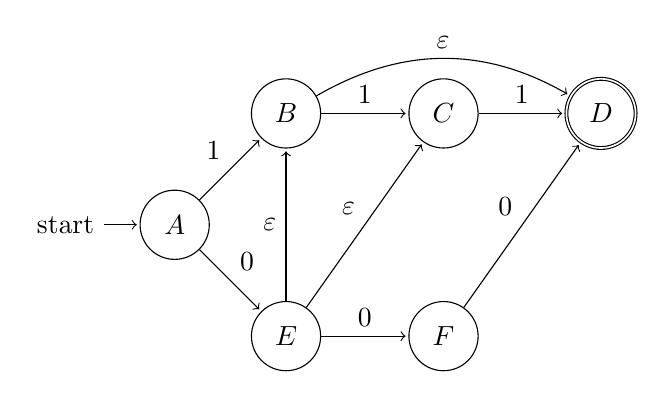
\begin{tikzpicture}[shorten >=1pt,node distance=2cm,on grid,auto]
  \node[state,initial]	(0)              		{$A$};
  \node[state]    			(1)   [above right  of=0] 	{$B$};
  \node[state]              (2)  [right of=1] 	{$C$};   
   \node[state,accepting]    			(3)   [right  of=2] 	{$D$};
    \node[state]    			(4)   [below right of=0] 	{$E$};
    \node[state]    			(5)   [right of=4] 	{$F$};

 \path[->]
     (0)	edge 	node	{1} (1)
        
     (1) edge node	{1} (2)
     (1) edge [bend left] node [above] {$\varepsilon$} (3)
     (2) edge node {1} (3)
     (0) edge node {0} (4)
     
     (4) edge  node {$\varepsilon$} (1)
     (4) edge node {$\varepsilon$} (2)
     (4) edge node {0} (5)
     (5) edge node {0} (3)
;
\end{tikzpicture}
\end{figure}
\end{frame}



\begin{frame}{Automate finite vs. Gramatici formale}
\begin{itemize}
\item
automatele finite, indiferent de tip, accepta numai limbaje regulare
\item
\textbf{automatele finite, indiferent de tip, au aceeași expresivitate ca și gramaticile regulare (sunt echivalente)}
\item
este foarte simplu de observat acest lucru, încercând să construim gramatica formală care defineşte acelaşi limbaj ca şi un AF dat
\item
se va observa că toate regulile de producţie ale gramaticii respective vor avea, cel puţin în forma iniţială, exact formatul cerut de definiția gramaticilor regulare
\end{itemize}
\end{frame}



\begin{frame}{Automate finite vs. Gramatici formale}
\textbf{De exemplu}, pentru AFD de mai jos, mulţimea regulilor de producţie a gramaticii care defineşte acelaşi limbaj ar putea avea elementele:

\begin{center}
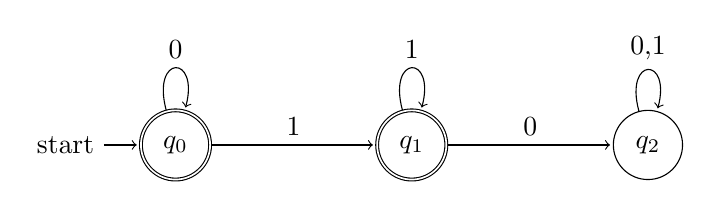
\begin{tikzpicture}[shorten >=1pt,node distance=3cm,on grid,auto]
\node[state,initial,accepting] (0) {$q_0$};
\node[state,accepting] (1) [right  of=0] {$q_1$};
\node[state] (2) [right of=1] {$q_2$};   

\path[->]
     (0) edge [loop above] node {0} (0)
         edge node {1} (1)
     (1) edge node {0} (2)
         edge [loop above] node	{1} (1)
	 (2) edge [loop above] node {0,1} (2)
	 ;
\end{tikzpicture}
\end{center}

\begin{itemize}
\item
$S \rightarrow 0S \ | \ 1P \ | \epsilon$
\item
$P \rightarrow 1P \ | \ 0Q \ | \epsilon$
\item
$Q \rightarrow 0Q \ | \ 1Q$
\end{itemize}
\end{frame}



\begin{frame}{Automate finite vs. Gramatici formale}
\textbf{Aplicaţie facultativă:}

\begin{itemize}
\item Implementarea într-un limbaj de programare oarecare a unei aplicaţii care să deducă gramatica formală echivalentă pentru un AFD dat.

\item Intrare: Pentru AFD se vor da, prin intermediul unui fişier de intrare, alfabetul, mulţimea stărilor, starea iniţială, mulţimea stărilor finale, tabelul de definiţie a funcţiei de tranziţie

\item Ieşire: Elementele de definiţie ale gramaticii formale echivalente.

\item Observaţii: 

\begin{itemize}
\item Alfabetul AFD va fi mulţimea terminalelor pentru G.

\item Mulţimea stărilor AFD va reprezenta mulţimea neterminalelor pentru G.

\item Starea iniţială va reprezenta simbolul de start pentru G.

\item Regulile de producţie se vor construi pe baza tranziţiilor AFD.
\end{itemize}
\end{itemize}
\end{frame}



\begin{frame}{Intrebari recapitulative}
\begin{itemize}

\item
Explicați la ce este folosită închiderea unei stări (closure) în cadrul algoritmului de eliminare a tranzițiilor epsilon ale unui automat finit epsilon.
\newline

\item
Explicați cum se folosește relația de mișcare pentru a defini limbajul acceptat de către un automat finit determinist.
\newline

\item
Explicați de ce este nevoie ca pentru automatele finite nedeterministe să se construiască automate finite deterministe echivalente.
\newline

\end{itemize}
\end{frame}



\begin{frame}{Intrebari recapitulative}
\begin{itemize}

\item
Care este restricția impusă numărului de elemente ale mulțimii stărilor din definiția unui automat finit nedeterminist, așa cum a fost introdusă la curs?
\newline

\item
Prezentați situațiile în care un automat finit epsilon este un automat finit determinist.
\newline

\item
Scrieți care este ultima configurație a șirului de relații de mișcare care reprezintă analiza sintactică ascendentă în baza unei gramatici $G$, efectuată de către un automat finit cu stivă pentru o propoziție care aparține lui $L(G)$.

\end{itemize}
\end{frame}



\begin{frame}{Intrebari recapitulative}
\begin{itemize}

\item
Fie automatul finit nedeterminist $A_1=(\Sigma, Q, F, q_0, f)$ și fie $A2=(\Sigma, Q', F', \{q_0\}, f')$ automatul finit determinist echivalent, obținut prin aplicarea algoritmului studiat. Scrieți ce relație există între $Q$ și $Q'$ și explicați.

\end{itemize}
\end{frame}




%%%%%%%%%%%%%%%%%%%%%%%%%%%%%%%%%%%%%%%%%%%%%%%%%%%%%%%%%%%%



\begin{frame}{Expresii regulare}
\textbf{Cuprins}
\begin{itemize}
\item
Expresii regulare
\item
Convenții de analiză pentru expresiile regulare
\item
De la expresii regulare la automate finite
\end{itemize}
\end{frame}



\begin{frame}{Expresii regulare}
\begin{itemize}
\item
Constituie un limbaj care permite descrierea altor limbaje (descrierea tuturor atomilor lexicali care pot aparea într-un limbaj).
\item
O expresie regulara R defineşte recursiv un limbaj L(R), astfel:
\begin{itemize}
\item
Şirul vid $\epsilon$ este o expresie regulara şi reprezinta şirul care nu conţine niciun caracter. 

\begin{center}
$L(\epsilon)=\{""\}$
\end{center}
\item 
Orice caracter singular $c$ este o expresie regulara şi reprezintă şirul de caractere, care conţine un singur caracter, şi anume pe $c$. 

\begin{center}
$L(c)=\{"c"\}$
\end{center}
\item 
\textbf{Concatenarea:} Daca $R_1$ şi $R_2$ sunt două expresii regulare, atunci $R1R2$ (citit $R_1$ concatenat cu $R_2$) este o expresie regulară şi reprezintă limbajul: 

\begin{center}
$L(R_1R_2)=\{s_1s_2| s_1 \in R1 \wedge s_2 \in R_2\}$
\end{center}
\end{itemize}
\end{itemize}
\end{frame}

\begin{frame}{Expresii regulare}
\begin{itemize}
\item
\textbf{Reuniunea:} Dacă $R_1$ şi $R_2$ sunt două expresii regulare, atunci $R_1|R_2$ este o expresie regulară şi reprezintă limbajul:

\begin{center}
$L(R_1|R_2)=L(R_1) \cup L(R_2)$.
\end{center}
\item
\textbf{Închiderea:} Dacă R este o expresie regulară, atunci $R^*$ este o expresie regulară şi reprezintă limbajul format din mulţimea de propoziţii obţinute prin concatenarea a zero sau mai multe şiruri, fiecare din $L(R)$. 

\begin{center}
$L(R^*) = L(\epsilon)\ \cup \ L(R)\ \cup\ L(RR)\ \cup\ L(RRR)\ \cup \dots$
\end{center}
\item
\textbf{Închiderea nereflexivă:} Dacă $R$ este o expresie regulară, atunci $R^+$ este o scriere prescurtată pentru $RR^*$.

\begin{center}
$L(R^+) = L(R) \cup L(RR) \cup L(RRR) \cup \dots$
\end{center}
\item
\textbf{Opţional:} Dacă $R$ este o expresie regulară, atunci $R?$ este o scriere prescurtată pentru $R|\epsilon$.
\end{itemize}
\end{frame}

\begin{frame}{Expresii regulare}
\textbf{Alte prescurtari permisei}

\begin{itemize}
\item
$[ c_{1} c_{2} \dots]$  este o prescurtare pentru  $c_{1} | c_{2} | \dots $.
\item
$a_{1}-a_{n}$ folosita intr-o prescurtare de tipul anterior reprezinta toate caracterele intre $a_{1}$  si $  a_{n} $.
\item
$[ \textasciicircum{} c_{1} c_{2}\dots]$ este o prescurtare pentru $d_{1}|d_{2}|\dots$, unde$ d_{1}, d_{2}, \dots$ sunt toate acele caractere care nu apar printre $c_{1}, c_{2}, \dots$.
\item 
$.$ este o prescurtare pentru toate şirurile de caractere care au un singur caracter, iar acesta nu este un terminator de linie.
\end{itemize}
\end{frame}

\begin{frame}{Expresii regulare}
\begin{itemize}
\item
Operatorii inchidere şi opţional au prioritate faţă de concatenare, care are prioritate faţă de reuniune.
\item
Pentru o scriere clară şi fără ambiguităţi se pot utiliza parantezele rotunde.

\item
Exemplu: Expresia regulara 

\begin{center}
$ab?cd*ef|g$ 
\end{center}

este echivalenta cu 

\begin{center}
$(a(b?)c(d*)ef)|g$
\end{center}

şi reprezintă limbajul format din propoziţiile : acef, g, acefg, abcef, abcefg, acdddef, acdddefg, abcdddefg, abcdddddef, s.a.m.d.
\end{itemize}
\end{frame}

\begin{frame}{Expresii regulare}
\begin{itemize} 
\item \textcolor{red}{Potrivirea unui text} 
	\begin{itemize}
	\item
	\textbf{Text}:    Anna Jones and a friend went to lunch 
	\item
	\textbf{Regex}:    went 
	\item
	\textbf{Matches}: Anna Jones and a friend \textbf{went} to lunch 
	\end{itemize}
	
\item \textcolor{red}{Potrivirea unui singur caracter oarecare (punct)}
	\begin{itemize}
	\item
	\textbf{Text}:       abc def ant cow 	
	\item
	\textbf{Regex}:    a.. 	
	\item
	\textbf{Matches}: \textbf{abc} def \textbf{ant} cow 
	\end{itemize}
	
\item \textcolor{red}{Potrivirea unui singur caracter dintr-un cuvânt (backslash w mic)}
	\begin{itemize}
	\item
	\textbf{Text}       abc anaconda ant cow apple 
	\item
	\textbf{Regex}:     a$\backslash$w$\backslash$w 
	\item
	\textbf{Matches}: \textbf{abc} \textbf{ana}conda \textbf{ant} cow \textbf{app}le
	\end{itemize}	
\end{itemize}
\end{frame}

\begin{frame}{Expresii regulare}
\begin{itemize} 
\item\textcolor{red}{Potrivirea unui singur caracter care nu este într-un cuvânt (backslash W mare)}
	\begin{itemize}
	\item
		\textbf{Text}:       abc anaconda ant cow apple
	\item
		\textbf{Regex}:      a\textbackslash W
	\item
		\textbf{Matches}:    abc anacond\textbf{a} ant cow apple
	\end{itemize}

\item\textcolor{red}{Potrivirea unui spaţiu alb (backslash s mic)}
	\begin{itemize}
	\item
		\textbf{Text}:	  abc anaconda ant
	\item
		\textbf{Regex}:    a\textbackslash w\textbackslash w\textbackslash s 
	\item
		\textbf{Matches}:  \textbf{abc} anaconda ant
	\end{itemize}
	
	Spaţiu alb este definit ca fiind caracterul spaţiu (\textbackslash 0x0020), new line (\textbackslash n), form feed (\textbackslash f), carriage return (\textbackslash r), tab (\textbackslash t) şi vertical tab (\textbackslash v).
\end{itemize}
\end{frame}

\begin{frame}{Expresii regulare}
\begin{itemize}
\item \textcolor{red}{Potrivirea unei cifre}
\begin{itemize}
\item \textbf{Text:} \space 123 12 843 8472
\item \textbf{Regex:} \space $\backslash d \backslash d \backslash d$
\item \textbf{Matches:} \textbf{123} 12 \textbf{843 847}2
\end{itemize}
\item \textcolor{red}{Potrivirea unui singur caracter dintr-un anumit set}
\begin{itemize}
\item \textbf{Text:} \space abc def ant cow
\item \textbf{Regex:} \space $[da]..$
\item \textbf{Matches:} \space \textbf{abc def ant} cow
\end{itemize}
\item \textcolor{red}{Adăugarea lui $\textasciicircum{}$ la începutul setului de caractere cere ca nici unul dintre caracterele din setul specificat să nu fie căutate}
\begin{itemize}
\item \textbf{Text:} \space abc def ant cow
\item \textbf{Regex:} \space $[\textasciicircum{} da]..$
\item \textbf{Matches:} \space a\underline{bc } d\underline{ef } a\underline{nt cow}
\end{itemize}
\end{itemize}
\end{frame}

\begin{frame}{Expresii regulare}
\begin{itemize}
\item \textcolor{red}{Potrivirea unui caracter dintr-o serie de caractere}
\begin{itemize}
\item
\textbf{Text}:	abc pen nda uml
\item
\textbf{Regex}:		.[a-d].
\item
\textbf{Matches}:	\textbf{abc} pen \textbf{nda} uml
\newline
\item
\textbf{Text}:		abc no 0aa i8i
\item
\textbf{Regex}:		[a-z0-9]\textbackslash w \textbackslash w
\item
\textbf{Matches}:	\textbf{abc} no \textbf{0aa i8i}
\end{itemize}

\item \textcolor{red}{Specificarea numărului de potriviri - de zero sau de mai multe ori}
\begin{itemize}
\item
\textbf{Text}: Anna Jones and a friend owned an anaconda
\item
\textbf{Regex}: a \textbackslash w\text{*}
\item
\textbf{Matches}: \textbf{Anna} Jones \textbf{and a} friend owned \textbf{an anaconda}
\end{itemize}

\item \textcolor{red}{Specificarea numărului de potriviri - o data sau de mai multe ori}
\begin{itemize}
\item
\textbf{Text}: Anna Jones and a friend owned an anaconda
\item
\textbf{Regex}: a \textbackslash w\text{+}
\item
\textbf{Matches}: \textbf{Anna} Jones \textbf{and} a friend owned \textbf{an anaconda}
\end{itemize}
\end{itemize}
\end{frame}

\begin{frame}{Expresii regulare}
\begin{itemize}
\item \textcolor{red}{Specificarea numărului de potriviri - de zero ori sau o data}
\begin{itemize}
\item
\textbf{Text:} Anna Jones and a friend owned an anaconda
\item
\textbf{Regex:} $an?$
\item
\textbf{Matches:} \textbf{An}n\textbf{a} Jones \textbf{an}d \textbf{a} friend owned \textbf{an} \textbf{a}cond\textbf{a}
\end{itemize}

\item \textcolor{red}{Specificarea exactă a numărului de potriviri}
\begin{itemize}
\item
\textbf{Text:} Anna Jones and Anne owned an anaconda
\item
\textbf{Regex:} $an\{2\}$
\item
\textbf{Matches:} \textbf{Ann}a Jones and \textbf{Ann}e owned an anaconda
\newline
\item
\textbf{Text:} Anna and Anne lunched with an anaconda annnnnex
\item
\textbf{Regex:}  $an\{2,3\}$
\item
\textbf{Matches:} \textbf{Ann}a and \textbf{Ann}e lunched with an anaconda \textbf{annn}nnex
\end{itemize}
\end{itemize}
\end{frame}

\begin{frame}{Expresii regulare}
\begin{itemize}
\item\textcolor{red}{ Potrivirea începutului unui şir}
\begin{itemize}
\item \textbf{Text:} an anaconda ate Anna Jones
\item \textbf{Regex:} $\wedge$a
\item \textbf{Matches:} \textbf{a}n anaconda ate Anna Jones
\end{itemize}
\item\textcolor {red}{Potrivirea sfârşitului unui şir}
\begin{itemize}
\item \textbf{Text:} an anaconda ate Anna Jones
\item \textbf{Regex:} \textbackslash w+\textdollar
\item \textbf{Matches:} an anaconda ate Anna \textbf{Jones}
\end{itemize}
\end{itemize}
\end{frame}

\begin{frame}{Convenţii de analiză pentru expresiile regulare}
\begin{itemize}
\item
În unele cazuri, secvenţe de caractere din codul sursă se pot potrivi la mai multe expresii regulare dintre cele folosite de către analizor.
\item 
Exemplu: Fie expresiile regulare: 

{\hfil (ab)* }

şi 

{\hfil [a-c]*}

Secvenţa de caractere "ab" se potriveşte ambelor expresii. 
\item
Deci \textbf{  trebuie convenit dacă expresiile au prioritate în ordinea apariţiei sau în ordinea inversă a apariţiei.}
\end{itemize}
\end{frame}

\begin{frame}{Convenţii de analiză pentru expresiile regulare}
\begin{itemize}
\item 
Pentru aceeaşi expresie regulară pot exista secvenţe de caractere diferite din codul sursă, care să se potrivească la un moment dat.
\item
Exemplu: Fie expresia regulară 

{\hfil ab|abcd}

şi şirul de intrare "abcd": se va extrage atomul "ab" sau atomul "abcd"?
\item 
Convenţie in acest sens  : \textbf {leftmost longest} - cea mai lungă secvenţă de caractere, citită de la stânga spre dreapta:
\begin{itemize}
\item
Pentru operatorii ?,*,+ se va lua secvenţa cea mai mare de caractere care se potriveşte subexpresiei din care fac parte şi care permite şi restului codului sursă să fie analizat.
\item
Dacă pentru o subexpresie $R_1|R_2$ se potriveşte o aceeaşi secvenţă de caractere, atunci se va lua  în considerare $R_1$.
\end{itemize}
\end{itemize}
\end{frame}

\begin{frame}{De la expresii regulare la automate finite }
\begin{itemize}
\item
\textbf{automatele finite și expresiile regulare au aceeași expresivitate (sunt echivalente)}
\item
orice expresie regulară poate fi convertită într-un automat finit
\item
construcţia automatului finit se face recursiv, pe baza definiţiei expresiei regulare
\item
pentru fiecare dintre expresiile regulare de bază, va fi prezentat automatul finit echivalent, cu o singură stare finală, folosind conventiile:
\begin{itemize}
\item
o elipsă reprezintă un automat, care recunoaşte expresia regulară R, sau aceeaşi maşină, dar cu toate stările componente transformate în stări nefinale
\item
o elipsă este o colecţie de stări şi tranziţii
\item
cele două stări marcate reprezintă starea iniţială şi respectiv starea finală, sau starea iniţială şi starea finală, transformată într-o stare nefinală
\end{itemize}
\end{itemize}
\end{frame}

\begin{frame}{De la expresii regulare la automate finite }
\begin{figure}
\begin{tabular}{c|c}
{$\epsilon$}&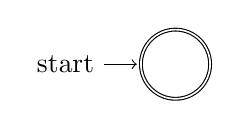
\begin{tikzpicture}[shorten >=1pt,node distance=2cm,on grid,auto]
  \node[state,initial,accepting]			(0)              			{$$};
\end{tikzpicture}  \\[6pt] \hline \\

a&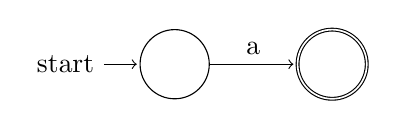
\begin{tikzpicture}[shorten >=1pt,node distance=2cm,on grid,auto]
  \node[state,initial]			(0)              			{$$};
  \node[state,accepting]              (1)   [right of=0] 		{$$};   

 \path[->]
     (0)	edge 			node	{a} (1)          
  ;
\end{tikzpicture} \\[6pt] \hline \\

$R_{1}$$R_{2}$&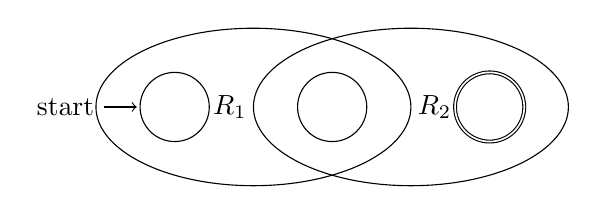
\begin{tikzpicture}[shorten >=1pt,node distance=2cm,on grid,auto]

  \node[state,initial]			(0)              			{$$};

  \node[state]    			(1)   [right  of=0] 	{$$};

\draw (1,0) ellipse(2cm and 1cm) node at (0.7,0){$R_{1}$};
\draw (3,0) ellipse(2cm and 1cm) node at (3.3,0){$R_{2}$};
  \node[state,accepting]    			(2)   [right  of=1] 	{$$};

\end{tikzpicture}\\[6pt] \hline \\

\end{tabular}
\end{figure}
\end{frame}

\begin{frame}{De la expresii regulare la automate finite}
\begin{figure}
\begin{tabular}{c|c}
$R_{1}$|$R_{2}$&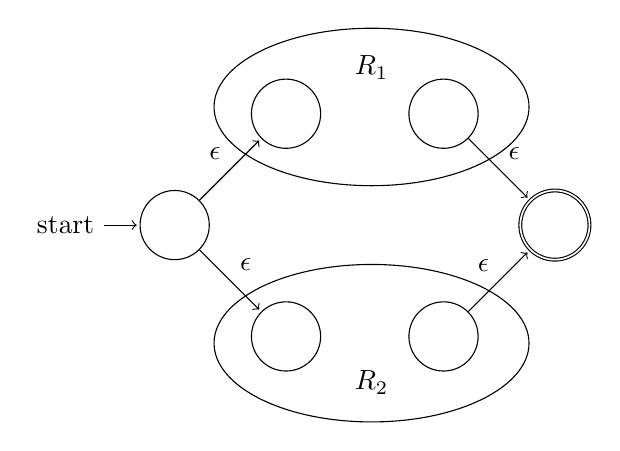
\begin{tikzpicture}[shorten >=1pt,node distance=2cm,on grid,auto]
  \node[state,initial]			(0)              			{$$};
\draw (2.5,1.5) ellipse(2cm and 1cm) node at (2.5,2){$R_{1}$};
  \node[state]    			(1)   [above right  of=0] 	{$$};
  \node[state]    			(2)   [below right  of=0] 	{$$};
  \node[state]    			(3)   [right  of=1] 	{$$};
  \node[state]    			(4)   [right  of=2] 	{$$};
\draw (2.5,-1.5) ellipse(2cm and 1cm) node at (2.5,-2){$R_{2}$};
  \node[state,accepting]              (5)   [below right of=3] 		{$$};   

 \path[->]
     (0)	edge 			node	{$\epsilon$} (2)
           edge			node	{$\epsilon$} (1)
     (3)	edge			node	{$\epsilon$} (5)
     (4)edge			node {$\epsilon$}(5)
  ;
\end{tikzpicture} \\[6pt] \hline \\

R*&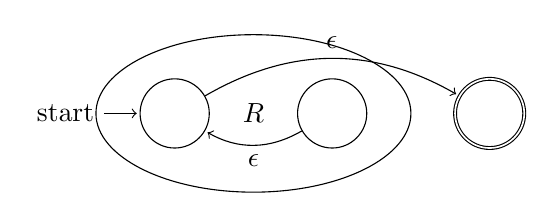
\begin{tikzpicture}[shorten >=1pt,node distance=2cm,on grid,auto]

  \node[state,initial]			(0)              			{$$};
\draw (1,0) ellipse(2cm and 1cm) node at (1,0){$R$};
  \node[state]    			(1)   [right  of=0] 	{$$};
  \node[state,accepting]    			(2)   [right  of=1] 	{$$};

\path[->]
     (0)	edge 	[bend left]		node	{$\epsilon$} (2)
     (1)edge [bend left]            	node {$\epsilon$} (0)
  ;
\end{tikzpicture}
  
\end{tabular}
\end{figure}
\end{frame}



\begin{frame}{De la expresii regulare la automate finite}
\begin{figure}
\begin{tabular}{c|c}
R+&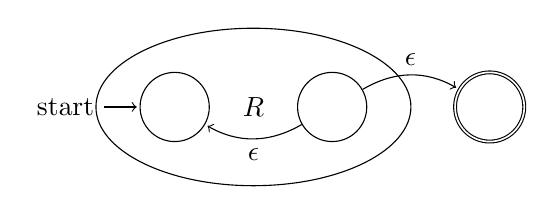
\begin{tikzpicture}[shorten >=1pt,node distance=2cm,on grid,auto]

  \node[state,initial]			(0)              			{$$};
  \draw (1,0) ellipse(2cm and 1cm) node at (1,0){$R$};
  \node[state]    			(1)   [right  of=0] 	{$$};
  \node[state,accepting]    			(2)   [right  of=1] 	{$$};

\path[->]
     (1)	edge 	[bend left]		node	{$\epsilon$} (2)
     (1)	edge 	[bend left]    	node 	{$\epsilon$} (0)
  ;
\end{tikzpicture}\\[6pt] \hline \\

$R?$&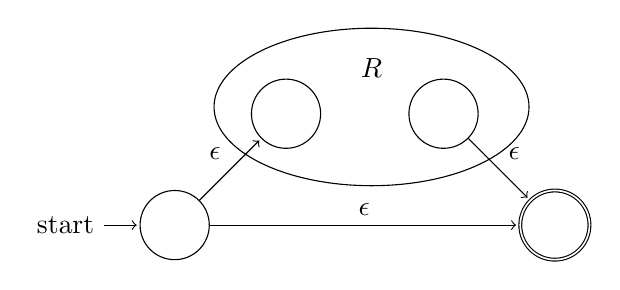
\begin{tikzpicture}[shorten >=1pt,node distance=2cm,on grid,auto]
  \node[state,initial]			(0)              			{$$};
	\draw (2.5,1.5) ellipse(2cm and 1cm) node at (2.5,2){$R$};
  \node[state]    			(1)   [above right  of=0] 	{$$};
  \node[state]    			(3)   [right  of=1] 	{$$};
  \node[state,accepting]              (5)   [below right of=3] 		{$$};   

 \path[->]
     (0)	edge 			node	{$\epsilon$} (5)
           	edge			node	{$\epsilon$} (1)
     (3)	edge			node	{$\epsilon$} (5)
  ;
\end{tikzpicture}
  
\end{tabular}
\end{figure}
\end{frame}



\begin{frame}{De la expresii regulare la automate finite}
\textbf{Aplicaţie facultativă}
\begin{itemize}
\item
Implementarea într-un limbaj de programare oarecare a unei aplicaţii care să construiască AFD care acceptă acelaşi limbaj ca şi o expresie regulară dată.
\item
Intrare: Expresia regulară.
\item
Iesire:
\begin{itemize}
\item
Elementele de definiţie ale AF-$\epsilon$ echivalent: alfabetul, mulţimea stărilor, starea iniţială, mulţimea stărilor finale, graful de tranziţie.
\item
Codul care implementează funcţionarea AFD echivalent pentru AF-$\epsilon$ de mai sus.
\end{itemize}
\end{itemize}
\end{frame}



\begin{frame}{Intrebari recapitulative}
\begin{itemize}

\item
Explicaţi ambiguităţile care pot să apară în utilizarea expresiilor regulare pentru a recunoaşte atomii lexicali dintr-un text dat.
\newline

\item
Fie $R$ o expresie regulară și fie expresiile regulare $R^*$ și $R^+$. Scrieți care este rezultatul operației $L(R^+)\setminus L(R^*)$ și explicați.
\newline

\item
Explicaţi care este diferenţa dintre un automat finit şi o expresie regulară relativ la definirea unui limbaj regular.
\newline

\end{itemize}
\end{frame}



%%%%%%%%%%%%%%%%%%%%%%%%%%%%%%%%%%%%%%%%%%%%%%%%%%%%%%%%%%%



\begin{frame}{Demonstrarea/infirmarea regularității unui limbaj}
\textbf{Cuprins}
\begin{itemize}
\item
Demonstrarea regularității unui limbaj
\begin{itemize}
\item
Construirea unui automat cu stări finite sau a unei expresii regulare
\end{itemize}
\item
Infirmarea regularității unui limbaj
\begin{itemize}
\item
Principiul cuiburilor de porumbei
\item
Lema pompării pentru limbajele regulare
\item
Teorema Myhill-Nerode à la Brzozowski
\end{itemize}
\end{itemize}
\end{frame}



\begin{frame}{Principiul cuiburilor de porumbei}
\begin{itemize}
\item
dacă \textit{n} porumbei zboară spre \textit{m} cuiburi şi dacă \textit{n>m}, atunci cel puţin un cuib va avea doi sau mai mulţi porumbei
\item
deoarece automatele finite au un număr finit de stări şi deoarece, în general,  există un număr infinit de propoziţii care sunt acceptate de către automat, atunci trebuie să existe cel puţin o stare la care automatul, în analiză, se întoarce de două sau de mai multe ori
\item
stările automatului sunt cuiburile, iar simbolurile propoziţiilor de la intrare sunt porumbeii
\end{itemize}
\end{frame}



\begin{frame}{Principiul cuiburilor de porumbei}
\begin{itemize}
\item
fie limbajul format din orice succesiune de 0 şi 1 care începe cu un 1, continuă apoi cu unul sau mai mulţi de zero, iar la sfârşit are un 1
\item
mulţimea propoziţiilor acestui limbaj este infinită, cuprinzând succesiunile de simboluri: $ 101 $, $ 1001 $, $ 10001 $, $ 10\dots01 $
\item
mulţimea stărilor automatului este finită
\item
conform principiului cuiburilor de porumbei, trebuie să există o stare $ q_m $ astfel încât, în analiza a două succesiuni de simboluri $ 10^{p} $ şi $ 10^{q} $, cu $ p \neq q $, automatul va ajunge în aceeaşi stare $ q_m $
\end{itemize}
\end{frame}



\begin{frame}{Principiul cuiburilor de porumbei}
\textbf{Exemplu}
\begin{itemize}
\item
$ L = \{ a^n b^n | n \geq 1  \} $
\item
presupunem că limbajul $ L $ este un limbaj regular
\item
înseamnă că există un automat finit $AF=(\{ a, b \}, Q, F, q_{0}, f)$ care acceptă acest limbaj
\item
considerăm $ f^* (q_0, a^i) $ pentru $ i $ egal cu $ 1, 2, \dots $
\item
deoarece $ i $, numărul de $ a $, poate lua un număr infinit de valori, şi deoarece mulţimea de stări din automat este finită, atunci, conform principiului cuiburilor de porumbei, există o stare $ q_k $ astfel încât:

$ f^* (q_0, a^m) = q_k $ şi $ f^* (q_0, a^n) = q_k $, cu $ m \neq n $.
\end{itemize}
\end{frame}



\begin{frame}{Principiul cuiburilor de porumbei}
\textbf{Exemplu}
\begin{itemize}
\item
deoarece automatul accepta şirurile de forma $ a^n b^n $, atunci este obligatoriu să fie adevărat că:

$ f^* (q_k, b^n) = q_f \in F $.
\item
pe baza relaţiile scrise mai sus, se poate deduce că:

$ f^* (q_0, a^m b^n) = f^* (f^* (q_0, a^m), b^n) = f^* (q_k, b^n) = q_f \in F$ 
\item
dar acest lucru înseamnă că automatul accepta şi şirurile de forma $ a^m b^n $, cu $ m \neq n $, ceea ce contrazice presupunerea iniţială cum că el accepta limbajul $ L $
\item
deci presupunerea iniţială este falsă şi deci $ L $ este un limbaj neregular
\end{itemize}
\end{frame}



\begin{frame}{Lema pompării pentru limbajele regulare}
Dacă L este un limbaj regular, atunci există un număr natural $N \geq 1$, astfel încât $\forall$ propoziţie w $\in$ L, unde |w| $\geq$ N, $\forall$ x, y, z astfel încât w=xyz, şi :
\begin{itemize}
\item
$|xy| \leq N$
\item
y $\neq$ $\epsilon$
\item
$\forall$ q $\geq$ 0, $xy^{q}z$ $\in$ L.
\end{itemize}
\end{frame}



\begin{frame}{Lema pompării pentru limbajele regulare}
\begin{itemize}
\item
dacă $ L $ este un limbaj regular, atunci înseamnă că există un automat finit determinist care îl defineşte
\item
presupunem că automatul are un număr $ n + 1 $ de stări şi că acestea sunt etichetate cu $ q_0, q_1, \dots, q_n $. 
\item
fie atunci o propoziţie $ w \in L $, astfel încât $ |w| \geq m = n +1 $ 
\item
fie $ q_0, q_i, q_j, \dots, q_f $ succesiunea de stări prin care automatul trece în analiza propoziţiei $ w $ (evident $ q_0 $ este starea iniţială, iar $ q_f $ este o stare finală)
\end{itemize}
\end{frame}



\begin{frame}{Lema pompării pentru limbajele regulare}
\begin{itemize}
\item
numărul de stări din cadrul acestei succesiuni de stări este egal cu lungimea şirului $ w $ plus 1, deoarece pentru a accepta un număr de simboluri egale cu lungimea lui $ w $, este nevoie de acelaşi număr de tranziţii, iar numărul de stări necesare pentru a forma aceste tranziţii este mai mare cu 1
\item
implică faptul că cel puţin o stare din succesiunea $ q_0, q_i, q_j, \dots, q_f $ se repetă
\item
prin urmare, succesiune de stări poate fi rescrisă $ q_0, q_i, q_j, \dots, q_r, \dots, q_r, \dots, q_f $
\end{itemize}
\end{frame}



\begin{frame}{Lema pompării pentru limbajele regulare}
\begin{itemize}
\item
această scriere a succesiuni de stări prin care trece automatul în analiza şi acceptarea propoziţiei $ w $, indică că aceasta poate fi scrisă ca o concatenare a trei subşiruri $ x, y, z $, astfel încât:
\begin{itemize}
\item
şirul $ x $ este prima parte a propoziţiei $ w $, pentru analiza căreia automatul trece prin succesiunea $ q_0, q_i, q_j, \dots, q_r$, şi se poate scrie:

$ (q_0,x) \vdash^* (q_r, \epsilon)  $ sau $ f^*(q_0, x) = q_r $
\item
şirul $ y $ este partea de mijloc a propoziţiei $ w $, pentru analiza căreia automatul trece prin succesiunea $ q_r, \dots, q_r$,  şi se poate scrie:

$ (q_r,y) \vdash^+ (q_r, \epsilon)  $ sau $ f^*(q_r, y) = q_r $
\item
iar şirul $ z $ este ultima parte a propoziţiei $ w $, pentru analiza căreia automatul trece prin succesiunea $q_r, \dots, q_f $, şi se poate scrie:

$ (q_r,z) \vdash^+ (q_f, \epsilon)  $ sau $ f^*(q_r, z) = q_f $
\end{itemize}
\end{itemize}
\end{frame}



\begin{frame}{Lema pompării pentru limbajele regulare}
\begin{itemize}
\item
rezultă că:

\begin{itemize}
\item
$ |xy| \leq n + 1 = m $ deoarece am presupus ca singura stare care se repetă în analiza propoziţiei $ w $ este $ q_r $ şi deci, în rest, stările sunt distincte

prin urmare, pentru şirurile $ x, y $ se pot analiza un număr maxim de simboluri egal cu numărul maxim de stări care pot fi implicate în analiză, adică $ n + 1 $;
\item
$ |y| \geq 1 $, deoarece s-a arătat că starea $ q_r $ trebuie să se repete, şi deci între cele două apariţii ale acestei stări va fi acceptat cel puţin un simbol (în cazul în care a doua apariţie a lui $ q_r $ urmează imediat după prima)
\end{itemize}
\end{itemize}
\end{frame}



\begin{frame}{Lema pompării pentru limbajele regulare}
\begin{itemize}
\item
având în vedere relaţiile de mai sus, se poate scrie că:

\begin{enumerate}
\item
$ (q_0,xz) \vdash^* (q_r, z) \vdash^+ (q_f, \epsilon) $, ceea ce înseamnă că $ xz \in L $;
\item
$ (q_0,xy^{2}z) \vdash^* (q_r, y^{2}z) \vdash^+ (q_r, yz) \vdash^+ (q_r, z) \vdash^+ (q_f, \epsilon)$, ceea ce înseamnă că $ xy^{2}z \in L $
\item
în acelaşi mod se poate arăta că $ xy^{3}z \in L $ şi $ xy^{4}z \in L $, şi, în general, $ xy^{q}z \in L $, pentru orice număr natural $ q $
\end{enumerate}
\end{itemize}
\end{frame}



\begin{frame}{Lema pompării pentru limbajele regulare}
\textbf{Exemplul 1}
\begin{itemize}
\item
L=\{$a^{n}$ $b^{n}$| n$\geq$ 1\}
\item
presupunem că limbajul este unul regular
\item
înseamnă că există un număr natural $N \ge 1$ astfel încât pentru orice propoziție $w \in L$ care are lungimea cel puțin egală cu $N$ se îndeplinesc afirmațiile lemei
\item
fie w = $a^{N}$ $b^{N}$
\item
atunci, indiferent de modul în care propoziția $w$ este scrisă ca și o concatenare de trei șiruri $xyz$, se îndeplinesc afirmațiile teoremei
\end{itemize}
\end{frame}



\begin{frame}{Lema pompării pentru limbajele regulare}
\textbf{Exemplul 1}
\begin{itemize}
\item
având în vedere
\begin{itemize}
\item
că în conformitate cu lema pompării, $|xy| \le N$ 
\item
felul în care l-am ales pe $w$
\end{itemize}
înseamnă că $y$ poate lua următoarele forme:

y=$a^{i}$, $1 \leq |y| \leq N$

\item
însă, pentru că $|xy| \leq N$:

$x=a^{j}$, cu condiția că $i+j \leq N$
\item
cu aceste observații, rezultă că șirul $w$ are forma:  

$w=a^{j}$ $a^{i}$ $a^{N-(i+j)}$ $b^{N}$
\end{itemize}
\end{frame}



\begin{frame}{Lema pompării pentru limbajele regulare}
\textbf{Exemplul 1}
\begin{itemize}
\item
în aceste condiții, lema afirmă că pentru orice număr natural $q \ge 0$, $x y^q z \in L$
\item
căutăm o valoare a lui $q$ astfel încât: 

$w^{`}$= $a^{j}$ ${a^{i}}^{q}$ $a^{N-(i+j)}$ $b^{N}$ $\nexists$ L, 

unde  $w^{`}$ este şirul pompat. 
\item
pentru $q=0$: 

$w^{`}$= $a^{j}$ $a^{N-(i+j)}$ $b^{N}$ = $a^{N-i}$ $b^{N} \notin L$
\item
contradicție: prin urmare, limbajul $L$ nu este un limbaj regular
\end{itemize}
\end{frame}



\begin{frame}{Lema pompării pentru limbajele regulare}
\textbf{Exemplul 2}
\begin{itemize}
\item
lema pompării nu poate fi folosită pentru a demonstra că un limbaj este regular, deoarece reciproca ei nu este adevărată: există limbaje care pot fi pompate, dar care, totuşi, nu sunt regulare
\item
L = \{ uvwxy : u,y $\in$ \{0,1,2,3\}* ; v, w, x $\in$ \{0,1,2,3\} $\wedge$ ( v = w $\vee$ v=x $\vee$ x=w ) \} $\cup$ \{ w : w $\in$ \{ 0,1,2,3 \}* $\wedge$  exact 1/7 simboluri din w să fie 3 \}
\item
limbajul nu este regular (spre exemplu $(013)^{3m}(012)^{i} \in L$ dacă și numai dacă $i=4m$), dar poate fi pompat pentru N având valoarea 5
\end{itemize}
\end{frame}



\begin{frame}{Lema pompării pentru limbajele regulare}
\textbf{Exemplul 2}
\begin{itemize}
\item
fie o propoziție $w$ care are lungimea cel puțin egală cu 5
\item
deoarece alfabetul limbajului are numai 4 simboluri, înseamnă că cel puțin două dintre primele 5 simboluri sunt identice, iar aceste două simboluri identice sunt separate de cel mult trei simboluri
\end{itemize}
\end{frame}



\begin{frame}{Lema pompării pentru limbajele regulare}
\textbf{Exemplul 2}
\begin{itemize}
\item
dacă cele două simboluri identice nu sunt separate de niciun simbol sau sunt separate de un singur simbol, atunci se poate pompa oricare dintre celelalte două simboluri din propoziție

\begin{itemize}
\item
$\textbf{aa}bcd$, $\textbf{a}b\textbf{a}cd$, $b\textbf{aa}cd$, $b\textbf{a}c\textbf{a}d$, $bc\textbf{aa}d$, $bc\textbf{a}d\textbf{a}$, $bcd\textbf{aa}$, etc.
\item
pentru prima varianta se poate pompa simbolul $c$ sau simbolul $d$
\item
$\textbf{aa}bc^q d$ sau $\textbf{aa}bcd^q$
\end{itemize}
\item
dacă cele două simboluri identice sunt separate de două sau de trei simboluri, atunci pot fi pompate două dintre simbolurile care le separă
\begin{itemize}
\item
$\textbf{a}bc\textbf{a}d$, $\textbf{a}bcd\textbf{a}$, $b\textbf{a}cd\textbf{a}$, etc.
\item
pentru prima varianta se poate pompa grupul $bc$
\item
$a(bc)^q ad$
\end{itemize}
\end{itemize}
\end{frame}



\begin{frame}{Teorema Myhill-Nerode à la Brzozowski}
\begin{itemize}
\item
\textbf{derivata unui limbaj $L$ în raport cu un simbol $c$} este un nou limbaj obținut prin aplicarea următoarelor două operații:

\begin{enumerate}
\item
se rețin toate propozițiile limbajului $L$ care încep cu simbolul $c$.
\item
se elimină simbolul $c$ din poate aceste propoziții.
\end{enumerate}

\item
derivata unui limbaj $L$ în raport cu un simbol $c$ se definește astfel:

$\frac{d}{ dc}$L = \{ v | cv $\in$ L \}

\item
exemple:
\begin{itemize}
\item
$\frac{d}{da}$ ab*a = b*a
\item
$\frac{d}{db}$ ab*a =$\emptyset$
\item
$\frac{d}{db}$ b*a = b*a
\end{itemize}
\end{itemize}
\end{frame}



\begin{frame}{Teorema Myhill-Nerode à la Brzozowski}
\begin{itemize}
\item
\textbf{derivata unui limbaj regular este tot un limbaj regular}
\item
orice limbaj regular poate fi definit prin intermediul unui automat cu stări finite
\item
dar, operația de derivare, prin care se obține limbajul derivat, corespunde schimbării stării inițiale a automatului finit care definește limbajul supus operației de derivare
\item
prin urmare și derivata unui limbaj este definită printr-un automat cu stări finite, ceea ce înseamnă că este un limbaj regular
\end{itemize}
\end{frame}



\begin{frame}{Teorema Myhill-Nerode à la Brzozowski}
\begin{itemize}
\item
\textbf{un limbaj regular are un număr finit de derivate distincte}
\item
având în vedere că 
\begin{itemize}
\item
operația de derivare a unui limbaj înseamnă de fapt schimbarea stării inițiale a automatului cu stări finite care definește limbajul supus derivării 
\item
numărul de stări ale unui automat este finit
\end{itemize}
\item
rezultă că numărul de derivate posibile este maxim egal cu numărul de stări ale automatului și deci este un număr finit
\item
reciproca afirmației este și ea adevărată: \textbf{dacă un limbaj are un număr finit de derivate distincte, atunci el este un limbaj regular}
\end{itemize}
\end{frame}



\begin{frame}{Teorema Myhill-Nerode à la Brzozowski}
\textbf{Exemplul 1}
\begin{itemize}
\item
L = \{ $a^{i} b^{i}$ | $\forall$ i $\in \mathbb{N}$ \}
\item
pentru a arăta că limbajul nu este regular, se va arăta că numărul de derivate distincte ale limbajului este infinit
\item
de exemplu, se va deriva limbajul dat în raport cu $a^n$
\item
$\frac{d}{da^{n}}$ $a^{i+n}$ $b^{i+n}$ = $a^{i}$ $b^{i+n}$, $\forall i,n \in \mathbb{N}$
\item
depinzând de $n$, este evident că numărul de derivate distincte obținute este infinit
\item
prin urmare, limbajul nu este regular
\end{itemize}
\end{frame}



\begin{frame}{Teorema Myhill-Nerode à la Brzozowski}
\textbf{Exemplul 2}
\begin{itemize}
\item
L = \{ $a^{i} b$ | $\forall$ i $\in \mathbb{N}$ \}
\item
$\frac{d}{da^{n}}$ $a^{i+n}$b = $a^{i}b $ 
\item
numărul de derivate este tot infinit, însă ele nu sunt distincte
\item
prin urmare limbajul este unul regular
\end{itemize}
\end{frame}



\begin{frame}{Teorema Myhill-Nerode à la Brzozowski}
\textbf{Exemplul 3}
\begin{itemize}
\item
L = \{ uvwxy : 

u,y $\in$ \{0,1,2,3\}*; 

v, w, x $\in$ \{0,1,2,3\} $\wedge$ ( v = w $\vee$ v=x $\vee$ x=w ) \} 

$\cup$ \{ w $\in$ \{0,1,2,3\}*| ( $n_{\{0,1,2\}}(w) = 6*n_{\{3\}} (w)$ \}
\item
notând cu $C$ a doua submulțime a propozițiilor din limbajul $L$, vom calcula derivata:
\item
$\frac{d}{d(0123)^{i}}$C 
\end{itemize}
\end{frame}



\begin{frame}{Teorema Myhill-Nerode à la Brzozowski}
\textbf{Exemplul 3}
\begin{itemize}
\item
= \{w $\in$ \{0123\}* | $n_{\{0,1,2\}}((0123)^{i}w) = 6*n_{\{3\}}((0123)^iw)$ \} 
\item
= \{w $\in$ \{0123\}* | $n_{\{0,1,2\}}((0123)^{i}) + n_{\{0,1,2\}}(w) = 6*(n_{\{3\}}((0123)^{i}) +  n_{\{3\}}(w)) \}$ 
\item
= \{w $\in$ \{0123\}* | $3*i + n_{\{0,1,2\}}(w) = 6*i + 6*n_{\{3\}}(w)$ \}
\item
= \{w $\in$ \{0123\}* | $n_{\{0,1,2\}}(w)  = 3*i + 6*n_{\{3\}}(w)$ \}
\item
aceste limbaje sunt distincte
\begin{itemize}
\item
spre exemplu, pentru fiecare valoare a lui $i$ derivata $\frac{d}{d(0123)^{i}}C$ conține șirul $(012)^i$
\item
însă niciuna dintre celelate derivate nu conține acest șir
\end{itemize}
\item
prin urmare, $L$ are un număr infinit de derivate distincte și deci nu este un limbaj regular
\end{itemize}
\end{frame}



\begin{frame}{Intrebari recapitulative}
\begin{itemize}

\item
De ce nu se poate folosi lema pompării pentru a demonstra că un limbaj este regular?
\newline

\item
Explicați care este diferența dintre reciproca lemei pompării și reciproca teoremei Myhill-Nerode à la Brzozowski.
\newline

\end{itemize}
\end{frame}



\begin{frame}{Intrebari recapitulative}
\begin{itemize}

\item
Explicați legătura dintre caracterul finit al mulțimii stărilor automatelor finite și Teorema Myhill-Nerode à la Brzozowski.
\newline

\item
Explicați rolul principiului cuiburilor de porumbei în înțelegerea limbajelor regulare.
\newline

\end{itemize}
\end{frame}



\begin{frame}{Intrebari recapitulative}
\begin{itemize}
\item
Fie $\Sigma$ alfabetul unui limbaj $L$, astfel încât $a, b, x$ $\in \Sigma$. Cunoscând că limbajul $L$ are proprietățile:

\begin{itemize}
\item
$ax \in L$ $\Leftrightarrow$ $bx \in L$,

\item
numărul de propoziții de forma $ax$ din $L$ este $k$.
\end{itemize}

Să se scrie care este rezultatul operației: 

card(L) – card(d/da L) – card(d/db L).
\newline

\end{itemize}
\end{frame}



%%%%%%%%%%%%%%%%%%%%%%%%%%%%%%%%%%%%%%%%%%%%%%%%%%%%%%%%%%%%%%



\begin{frame}{Implementarea automatelor finite deterministe}
\textbf{Cuprins}
\begin{itemize}
\item
Exemplificare la tablă
\end{itemize}
\end{frame}



\begin{frame}{Bibliografie}
\begin{itemize}
\item
Halvor Eifring, Rolf Theil, Linguistics for Students of Asian and African Languages, Oslo, 2005
\url{https://www.uio.no/studier/emner/hf/ikos/EXFAC03-AAS/h05/larestoff/linguistics/}
\item
Paul Kay, Willett Kempton, What is the Sapir-Whorf hypothesis?, 1984
\url{http://www.blutner.de/color/Sapir-Whorf.pdf}
\item
Umberto Eco, “Limbajul Pământului Austral”, “De la arbore la labirint”, editura POLIROM, 2009.
\item
Vlad Tarko, The Metaphysics of Object Oriented Programming
\url{http://news.softpedia.com/news/The-Matephysics-of-Object-Oriented-Programming-24906.shtml}
\item
Wikipedia, Programming paradigm
\url{http://en.wikipedia.org/wiki/Programming\_paradigm}
\end{itemize}
\end{frame}


\begin{frame}{Bibliografie}
\begin{itemize}
\item
Irina Athanasiu, Limbaje formale și translatoare, 2002
\url{http://www.scribd.com/doc/22056333/Limbajeformale-\%C5\%9Fi-automate}
\item
Online regular expression designers
\begin{itemize}
\item
\url{https://www.debuggex.com/}
\item
\url{http://www.regexr.com}
\end{itemize}
\item
Regular Expressions to Non-Deterministic Finite Automata
\url{http://hackingoff.com/compilers/regular-expression-to-nfa-dfa}
\item
Bosker Blog, I hate the Pumping Lemma
\url{https://bosker.wordpress.com/2013/08/18/i-hate-the-pumping-lemma/}
\end{itemize}
\end{frame}



\end{document}